\documentclass[12pt,twoside]{article}

\usepackage[T1]{fontenc}
\usepackage[utf8]{inputenc}
\usepackage[spanish]{babel}

\let\layoutspanish\relax
\addto\captionsspanish{\def\tablename{Tabla}}
\unaccentedoperators

\usepackage[a4paper]{geometry}
  \geometry{hmargin={2.5cm,2.5cm},height=22cm}
  
\renewcommand{\baselinestretch}{1.2}  
\setlength{\partopsep}{0pt}
\setlength{\itemsep}{0pt}
\setlength{\topsep}{0pt}
\setlength{\parsep}{0pt}
\setlength{\parskip}{0.25\baselineskip}

\renewcommand{\textfraction}{0.1}
\renewcommand{\topfraction}{1}
\renewcommand{\bottomfraction}{1}
\renewcommand{\floatpagefraction}{1}

\setcounter{totalnumber}{5}
\setcounter{topnumber}{3}
\setcounter{bottomnumber}{2}

\usepackage{caption}


\usepackage{indentfirst}

\usepackage[pdftex]{color}
\usepackage[table,xcdraw]{xcolor}
\usepackage{float}

\usepackage[pdftex]{graphicx}

\usepackage{amsmath}
\allowdisplaybreaks 
\usepackage{amssymb}
\usepackage{amsfonts} 
\usepackage{enumerate}

\usepackage{fancyhdr}

\newcommand{\RunningAuthor}{Ginés Meca Carbonell}
\newcommand{\Author}[1]{\renewcommand{\RunningAuthor}{#1}}
\renewcommand{\leftmark}{\RunningAuthor}

\newcommand{\RunningTitle}{Métodos de Machine Learning basados en Árboles de Decisión.}
\newcommand{\Title}[1]{\renewcommand{\RunningTitle}{#1}}
\renewcommand{\rightmark}{\RunningTitle}

\pagestyle{fancy}
\fancyhf{}
\fancyhead[LO]{\small \slshape \leftmark}    
\fancyhead[RE]{\small \slshape \rightmark}   
\fancyhead[RO,LE]{\small \slshape \thepage}  

\renewcommand{\headrulewidth}{0.6pt}         
\renewcommand{\footrulewidth}{0pt}           
                                             
\setlength{\headheight}{1.5\headheight}      

\fancypagestyle{plain}{%                     
  \fancyhf{}                                 
  \setlength{\headwidth}{\textwidth}
  \fancyfoot[C]{\small \slshape \thepage}    
  \renewcommand{\headrulewidth}{0pt}
  \renewcommand{\footrulewidth}{0pt}
  }
  
\newcommand{\abs}[1]{\ensuremath{|#1|}}

\usepackage{hyperref}

\title{Métodos de Machine Learning basados en Árboles de Decisión}
\author{Ginés Meca Carbonell\\*[1em]
\begin{minipage}{0.75\textwidth}
\footnotesize \itshape
\begin{center}
Universidad de Alicante \\
4º de Grado en Matemáticas
\end{center}
\end{minipage}
}
\date{Julio 2022}

\usepackage{pdfpages}




\begin{document}


\includepdf[pages=1]{anexo-1-portada-memoria-tfg-matematicas.pdf}



\section*{Resumen}

\emph{En este trabajo, se ha estudiado el conjunto de algoritmos de Machine Learning que derivan de los árboles de decisión, confeccionando un mapa conceptual de modelos de manera que podamos clasificarlos en cuanto a aspectos teóricos y reconocer sus principales características. Los árboles de decisión son algoritmos capaces de aprender de variables explicativas de datos conocidos y realizar predicciones sobre datos nuevos. Mediante diferentes tipos de combinaciones, se llegan a dos grandes familias de modelos más complejos: algoritmos de bagging y algoritmos de boosting. Estos modelos de mayor complejidad son capaces de conseguir un significativo aumento de precisión, especialmente cuando se enfrentan a grandes cantidades de datos. Por ello, son muy utilizados e imprescindibles actualmente para trabajar en Big Data.}

\emph{Para poder profundizar y realizar un correcto análisis de los modelos más complejos, en la primera parte se ha estudiado el proceso de construcción de árboles de decisión. En particular, se ha analizado el algoritmo CART, que es el más utilizado. A lo largo de esta sección, se introducen diferentes nociones como los criterios de escisión, los criterios de parada o la asignación de valores de respuesta. No obstante, dado que esta sección ya se ha tratado en varios trabajos de años anteriores, se ha decidido no profundizar en exceso para poder invertir un mayor tiempo en aquello que resulta novedoso.}

\emph{En la segunda parte del trabajo, se han estudiado los algoritmos de bagging y boosting por separado. Respecto a los algoritmos de bagging, se han explicado las ideas principales de su funcionamiento, ya que estos algoritmos también han sido tratados en cursos anteriores. En cuanto a los algoritmos de boosting, se ha realizado un detallado análisis de cada uno de ellos, explicando cuáles son las funciones y parámetros implicados así como el proceso exacto para conseguir disminuir el 
error de predicción.}

\emph{Por último, tras la explicación de cada tipo de algoritmo, se ha realizado un ejemplo práctico a fin de ilustrar aquello explicado de manera teórica. También, se han utilizado estos ejemplos para realizar una comparación en términos de precisión y tiempo computacional de todos los modelos explicados, señalando diferencias entre ellos y comprobando que se cumplen ciertas características previamente explicadas.}

\textbf{Palabras clave:} CART, Bagging, Boosting, Machine Learning



\newpage



\section*{Abstract}

\emph{In this research, it has been studied the set of Machine Learning algorithms derived from decision trees, making a conceptual map of models so that we can classify it according to their theoretical aspects and we can recognize their main features. Decision trees are algorithms capable of learning from known data explanatory variables and making predictions about new data. Through different types of combinations, we obtain two families of more complex models: bagging algorithms and boosting algorithms. These models are able to increase significatively the accuracy, specially when they have to deal with large amounts of data. That's why they are very useful models and they have become essential in Big Data technologies.}

\emph{In order to study in more detail and analyze correctly the complex models introduced, in the first part of this work it has studied the decision trees building process. In particular, it has been analyzed the most popular algorithm: CART. Along this section, different notions like split criterions, stop criterions or output assignment are introduced. Nevertheless, since this topic has been explained in previous researches we have not focused on it, in order to spend more time on the new algorithms introduced.}

\emph{In the second part of this work, it has studied bagging and boosting algorithms by separate. In regard to bagging algorithms, it has been explained the main ideas related to their functioning, since these algorithms have been treated in former works too. Referring to boosting algorithms, it has been done a complete analysis of each of them, explaining which are the functions and parameters implied as well as the exact process applied to reduce the prediction error.}

\emph{Finally, after each type of algorithms explanation, solve a practical example has been solved in order to illustrate what the theory explained. Furthermore, these examples have been used to make a accuracy and running time comparison of all models, showing the differences between them and checking the features explained previously.}

\textbf{Key words:} CART, Bagging, Boosting, Machine Learning



\newpage



\tableofcontents



\newpage



\section{Introducción}

Vivimos en la era de la información. Cada segundo, millones de datos viajan entre diferentes lugares del planeta y se guardan formando enormes conjuntos de datos. Además, cada vez hay más instrumentos capaces de recoger información. Donde antes se necesitaba hacer uso de encuestas, ahora nos encontramos con dispositivos, como los teléfonos móviles, capaces de escribir texto, recoger audio y realizar fotografías y vídeos. Así, la información a nuestra alcance es infinita. Podemos conocer cuáles son los conceptos que son tendencia en los buscadores de internet, o cuáles son aquellos audiovisuales que más éxito están teniendo en las redes sociales. Del mismo modo, podemos acceder al historial de imágenes de la cámara de seguridad de nuestra vivienda o a la tabla que recoge las últimas operaciones de nuestra empresa. Es fácil obtener grandes cantidades de datos de aquello que nos interesa.

Dado que el número de datos que manipulamos cada vez es mayor,las técnicas utilizadas para analizarlos van evolucionando constantemente. Muchas de las técnicas clásicas del análisis de datos han quedado obsoletas, otras se utilizan para crear algoritmos más complejos. Uno de los algoritmos más conocidos es el de los árboles de decisión. Fueron introducidos por primera vez en 1963 por James N. Morgan y John A. Sonquist \cite{MO01}, quienes obtuvieron un método muy eficaz a través de un algoritmo muy básico. Actualmente, existen diferentes algoritmos que se pueden emplear a la hora de generar un árbol de decisión: CHAID, C4.5, FACT, QUEST, CRUISE... No obstante, el más conocido, y el que estudiaremos en este trabajo, es el algoritmo CART (Classification And Regression Trees), creado por Breiman, Friedman, Olshen y Stone en 1984 \cite{BR03}. De hecho, fue el propio Leo Breiman quien, haciendo uso de CART, desarrolló años más tarde algoritmos como Bagging \cite{BR01} Random Forest \cite{BR02}. Paralelamente, la publicación de Freund y Schapire en 1997 \cite{FR01} de un nuevo método basado en boosting daría lugar a otra serie de algoritmos, donde nos encontramos algoritmos más complejos, como XGBoost, que ocuparán gran parte del trabajo.

Dado que en los últimos años varios alumnos han realizado su TFG sobre árboles de decisión explicando su estructura más básica, resumiré las secciones dedicadas a ello con el fin de centrarme en analizar a fondo los algoritmos más complejos y novedosos que no se han tratado en estos trabajos y, así, lograr elaborar un mapa conceptual de modelos lo más completo posible.



\subsection{Datos: Llueve en Australia} \label{sec: subsec11}

Para hacernos una idea de cómo funciona cada uno de los algoritmos explicados a lo largo del trabajo, haremos uso del conjunto de datos ``Rain in Australia'', de Kaggle. Se trata de un dataset en el que podemos encontrar mediciones de diferentes variables meteorológicas así como la fecha y localidad correspondientes y la información relativa a si llovió o no el día de la medición y el día siguiente. Así, el objetivo será averiguar si con los datos del día actual se puede predecir si lloverá el día siguiente utilizando los diferentes algoritmos descritos. 
\begin{figure}[h]
	\centering
	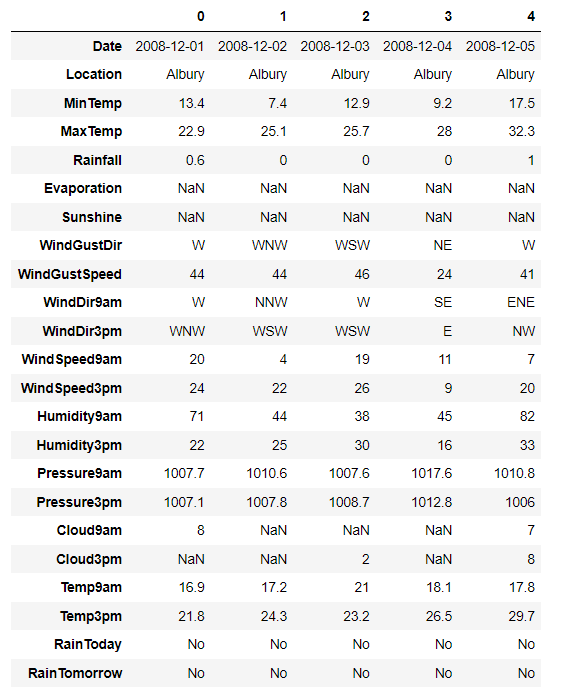
\includegraphics[width = 0.4\textwidth]{Intro_01}
	\caption{Encabezado del dataset}
\end{figure}

En resumen, se tienen 23 columnas que recogen información de un total de 145.460 días. En los diferentes ejemplos, se tratará de realizar predicciones de la variable ``Rain Tomorrow''.


\subsection{Metodología} \label{subsec:Metodología}

A la hora de aplicar los diferentes métodos al conjunto de datos se procederá mediante validación cruzada. Es decir:

\begin{enumerate}
\item Se selecciona el modelo correspondiente.
\item Se separa, al azar, el conjunto de datos inicial en dos: datos de entrenamiento y datos de testeo.
\item Se entrena el modelo con los datos de entrenamiento.
\item Se aplica el modelo entrenado a los datos de testeo.
\item Se comprueba la precisión de las predicciones realizadas.
\end{enumerate}

Habitualmente, la división del conjunto inicial que da lugar a los subconjuntos de entrenamiento y testeo se realiza de manera aleatoria. No obstante, dado que los datos podrían interpretarse como una serie temporal, donde se recogen mediciones diarios a lo largo de 10 años, a la hora de realizar predicciones sobre las posibles variables de interés nos interesa conocer la la precisión de nuestro modelo ante datos futuros.  Así, realizar una división aleatoria del conjunto incial conllevaría que los datos de entrenamiento se encontrarían intercalados con los de testeo por lo que no sabríamos determinar la fiabilidad real del modelo, pues estas predicciones no nos aportarían ningún tipo de información acerca de la precisión del algoritmo a la hora de clasificar datos de fechas posteriores.

Por tanto, el procedimiento será ligeramente distinto. Emplearemos una validación \textit{``Out Of Time''}, basada en separar el conjunto de datos siguiendo un orden cronológico. Dado que nuestro dataset contiene fechas desde el 01/11/2007 hasta el 24/06/2017, nuestro conjunto de entrenamiento estará formado por todos aquellos datos con fecha anterior al 01/01/2015 y los datos de testeo serán los restantes. Así, entrenamos el modelo con datos anteriores a los de testeo para saber cómo van a ser las predicciones futuras y asemejarnos más a lo que nos interesaría en un caso real: entrenar el modelo en función de los datos que poseemos para predecir fechas futuras.

Además, los cálculos se realizarán en el lenguaje de programación Python. Todo el código se encuentra disponible en el Anexo (\ref{Anexo}), publicado en GitHub.



\newpage



\section{Árboles de decisión CART}
\subsection{Preliminares}

Los árboles de decisión son muy utilizados como método predictor (tanto de regresión como de clasificación) dada su simpleza, su efectividad y lo visual que resulta su funcionamiento a través de un gráfico, lo cual facilita su comprensión. También, se pueden utilizar como herramienta descriptiva para un entendimiento inicial de los datos de un proyecto. Se trata de un algoritmo que divide sucesivamente de manera lineal el conjunto de datos inicial en diferentes subconjuntos a través de diversas condiciones aplicadas a sus variables explicativas. Por ejemplo:

\textbf{Ejemplo 2.1: } \label{Ej:2.1} \emph{Se pretende estudiar la variable ``RainTomorrow'' del conjunto de datos dado en función de las variables explicativas ``Cloud3pm'' y ``Humidity3pm''(nivel de nubosidad y de humedad a las 15.00, respectivamente) para predecir si lloverá o no al día siguiente. Así, escogiendo únicamente las variables explicativas indicadas, el esquema que ha aprendido el árbol de clasificación es el siguiente: }
\begin{figure}[h]
	\centering
	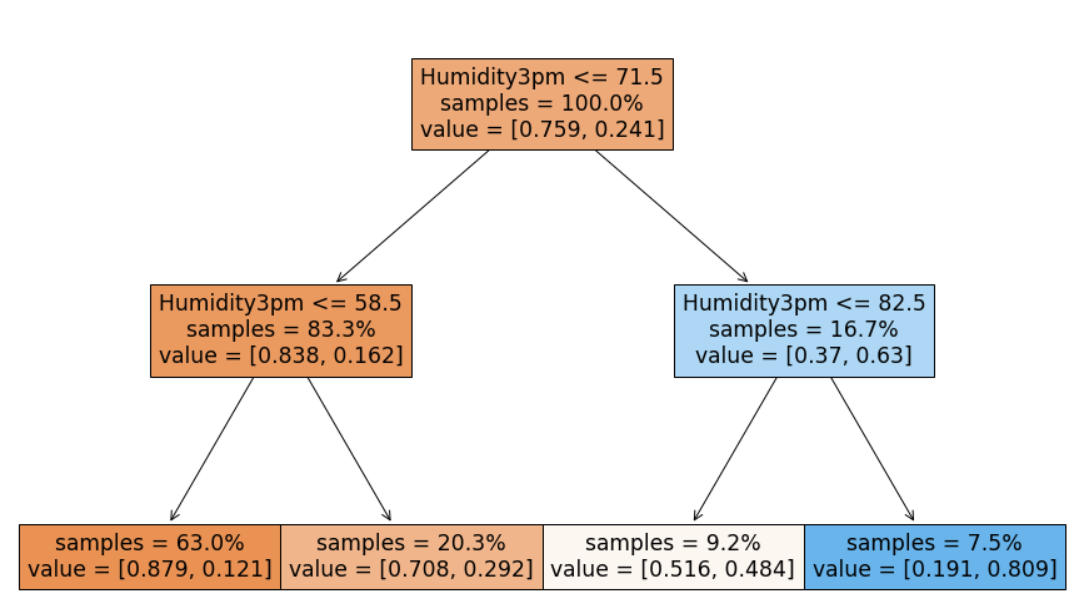
\includegraphics[width = 0.7\textwidth]{ex2_1_01}
	\caption{Árbol de decisión del Ejemplo \ref{Ej:2.1}}
	\label{fig:Ejemplo 2.1}
\end{figure}

Como se puede observar, el algoritmo es muy intuitivo: se introduce un individuo y se le aplica la primera condición; si la respuesta es afirmativa se sigue el camino de la izquierda y si es negativa el de la derecha. Mediante este proceso, se va comprobando si sus variables explicativas cumplen las diferentes condiciones que se plantean hasta alcanzar un grupo al que no se le aplican condiciones, el cual determinará su predicción.

Por otro lado, es fácil ver que las condiciones del algoritmo se corresponden con particiones del espacio. Como en el ejemplo anterior se han elegido únicamente dos variables explicativas, se puede hacer una representación de los individuos sobre $\mathbb{R}^{2}$ y determinar sobre él las diferentes regiones de predicción.
\begin{figure}[h]
	\centering
	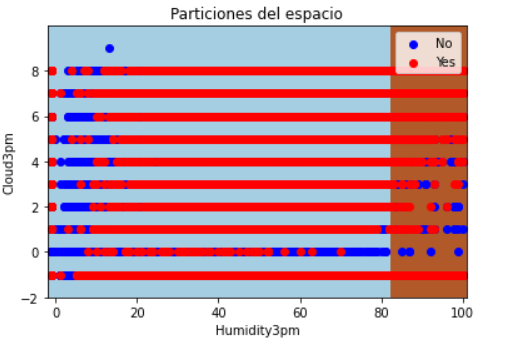
\includegraphics[width = 0.5\textwidth]{ex2_1_02}
	\caption{Partición del espacio del Ejemplo \ref{Ej:2.1}}
	\label{fig:Ejemplo 2.1.2}
\end{figure}


\subsubsection{Notación y conceptos básicos}

A continuación, se introducen una serie de términos básicos para poder hacer referencias correctas a los conceptos presentados. Por un lado, nos encontramos con las siguientes definiciones:
\begin{description}
\item[Nodo raíz: ]Primer nodo, contiene a todos los individuos y a partir de él comienzan a realizarse las divisiones.
\item[Nodo interno: ]Nodos intermedios que provienen de una división y desencadenan otra. Dentro de ellos, se pueden definir:
	\begin{description}
	\item[Nodo padre: ]Nodo anterior a un nodo interno fijado.
	\item[Nodos hijos: ]Nodos resultantes de la división del nodo interno fijado.
	\end{description}
\item[Nodo hoja: ]Nodos finales que dan lugar a la predicción.
\end{description}

Todos estos elementos son fácilmente identificables en la figura \ref{fig:Ejemplo 2.1} del ejemplo 2.1 . Se tiene un nodo raíz, seis nodos internos y 8 nodos hoja.

Por otro lado, conviene hablar del concepto de sobreajuste (en inglés: \textit{overfitting}). Se dice que un modelo se encuentra sobreajustado si el algoritmo se ha adaptado en exceso a los individuos del conjunto de entrenamiento. Este hecho provoca que la predicción de los individuos de este conjunto sea muy buena, pero que las predicciones de nuevos individuos presenten grandes errores.

Para lidiar con el sobreajuste, interesa manejar otras dos nociones: el sesgo y la varianza. El sesgo (en inglés: bias) hace referencia a los errores cometidos en las predicciones de los individuos de nuestro conjunto de entrenamiento. Por contra, la varianza es la medida del error cometido en los individuos que no pertenecen a este conjunto; en nuestro caso, lo mediremos en los individuos del conjunto de testeo. No obstante, estos conceptos plantean un problema: interesa tener valores bajos de ambos indicadores, pero disminuir el sesgo conlleva un aumento de la varianza. Así, a la hora de construir un modelo de Machine Learning, interesa estudiar que el sesgo no sea excesivamente bajo, para evitar el sobreajuste, pero también que no sea excesivamente alto para que las predicciones sean fiables.


\subsubsection{Objetos de estudio de un CART}

Una vez explicada, de manera intuitiva, la manera de proceder de los árboles de decisión, corresponde explicar el verdadero funcionamiento de los mismos. Para ello, habrá que tratar los siguientes aspectos:
\begin{enumerate}
\item Elección de variables y valores asociados a cada nodo interno.
\item Criterio de parada de división de los nodos
\item Valor o clase asignada a cada nodo
\end{enumerate}



\subsection{Valor o clase asignada a cada nodo hoja} \label{sec:2.4}
Sea un conjunto de datos de n individuos y p+1 variables ($n,p \in \mathbb{N}$). De este modo, sean $X_1, X_2, ... , X_p$ las variables explicativas e $y$ la variable dependiente. En el caso de nuestro conjunto de datos de ejemplo:
\begin{table}[h]
\centering
\begin{tabular}{l|l|l|l|l|l|}
\cline{2-6}
                                                       & \cellcolor[HTML]{C0C0C0}$X_1$ & \cellcolor[HTML]{C0C0C0}$X_2$ & \cellcolor[HTML]{C0C0C0}$\dots$ & \cellcolor[HTML]{C0C0C0}$X_{22}$ & \cellcolor[HTML]{9B9B9B}$y$ \\ \hline
\multicolumn{1}{|l|}{\cellcolor[HTML]{C0C0C0}$x_1$}    & 2008-12-01                    & Albury                        & $\dots$                         & No                               & No                          \\ \hline
\multicolumn{1}{|l|}{\cellcolor[HTML]{C0C0C0}$x_2$}    & 2008-12-02                    & Albury                        & $\dots$                         & No                               & No                          \\ \hline
\multicolumn{1}{|l|}{\cellcolor[HTML]{C0C0C0}$_3$}     & 2008-12-02                    & Albury                        & $\dots$                         & No                               & No                          \\ \hline
\multicolumn{1}{|l|}{\cellcolor[HTML]{C0C0C0}$\vdots$} & $\vdots$                      & $\vdots$                      & $\ddots$                        & $\vdots$                         & $\vdots$                    \\ \hline
\end{tabular}
\caption{Datos \textit{``Rain in Australia''}}
\label{tab:Datos}
\end{table}

Como se comentaba anteriormente, el resultado de un árbol de decisión es una partición del espacio. Supongamos que se obtienen $M$ regiones diferentes, denotadas por $R_{m}$ con $m = 1, ..., M$. Por tanto, definamos como Y al árbol de decisión y como $c_m$, con $m = 1,...,M$, a las predicciones (imágenes de Y) asociadas a cada región $R_m$. De este modo:
\begin{equation*}
Y(x) = \sum^M_{m = 1} c_{m}I(x \in R_m) \, \, \, \forall x \in D
\end{equation*}

\noindent
donde D es el dominio de la función (espacio de las variables explicativas) e I es la función indicadora:
\begin{equation*}
I(x) = 
\left\{
\begin{array}{ccc}
1 & si & x \in R_m \\
0 & si & x \not\in R_m 
\end{array}
\right.
\end{equation*}

La manera de establecer el valor de estas predicciones presenta ligeras diferencias en función del tipo de problema con el que tratemos (regresión o clasificación). Por tanto, lo analizaremos por separado.


A la hora de entrenar un modelo de regresión, se busca minimizar los errores entre $y$ e $Y$. Tomando el error mínimo cuadrático, llegamos al problema:
\begin{equation*}
\min_{Y_i} \sum_{i=1}^n (y_i - Y_i)^2 \Rightarrow \min_{c_m} \sum_{m = 1}^M \sum_{x_i \in R_m} (y_i - c_m)^2
\end{equation*}

\noindent
donde $Y_i = Y(x_i) \, \, \forall i=1,...n$. Si denotamos $f(c_m) = \sum_{x_i \in R_m} (y_i - c_m)^2$, observamos que alcanzar la solución óptima del problema planteado es equivalente a minimizar la función f. Derivando, obtenemos un candidato a óptimo:
\begin{equation*}
f'(c_m) = -2 \sum_{x_i \in R_m} (y_i - c_m) = -2 \sum_{x_i \in R_m}y_i + 2n_mc_m = 0 \Leftrightarrow c_m = \frac{1}{n_m} \sum_{x_i \in R_m}y_i
\end{equation*}

\noindent
y se comprueba que, efectivamente, es el óptimo a través de la segunda derivada:
\begin{equation*}
f''(c_m) = -2 \sum_{x_i \in R_m} (-1) = 2n_m > 0
\end{equation*}

\noindent
donde $n_m$ es el conjunto de datos pertenecientes a la región $R_m$, $\forall m = 1,...M$.

En conclusión, el valor asignado a cada nodo hoja será la media de las observaciones de los individuos del conjunto de entrenamiento que pertenecen a dicho nodo.

En el caso de árboles de clasificación, la tarea se simplifica: basta con calcular la proporción de individuos de cada clase en cada región y, así, el valor asignado a cada subconjunto del espacio será la clase a la que le corresponde la mayor proporción en el mismo.


\subsection{Elección de variables y valores asociados a cada nodo interno} \label{sec: subsec22}

Pese a las similitudes existentes entre los árboles de regresión y los de clasificación, conviene dividir este apartado en dos con tal de mostrar el funcionamiento exacto de cada uno de ellos.


\subsubsection*{Árboles de regresión}
Se busca conocer cómo realizar las divisiones. En particular, nos centraremos en la primera división y el proceso será similar para las siguientes. Al situarnos en el nodo raíz, nos encontramos con el conjunto de datos al completo y pretendemos dividirlo en dos regiones, que denotaremos $R_1$ y $R_2$, en función de una de las variables explicativas, $X_j$, y de un valor respecto de esta, $s$, de manera que cada región contendrá a los individuos:
\begin{equation*}
R_1 (j,s) = \{ x_i | x_{ij} \leq s \} \, \, \, \wedge \, \, \,  R_2 (j,s) = \{ x_{i} | x_{ij} > s\}
\end{equation*}

Así, se generan dos valores de predicción constantes, uno por cada nodo hoja; es decir, se definen $c_1$ y $c_2$ tales que $c_1$ se mantendrá constante sobre $R_1$ e $c_2$ constante sobre $R_2$. Ya hemos visto que estos $c_m$ se corresponderán con la media de los individuos del nodo hoja:
\begin{equation*}
c_m = \frac{1}{n_m}\sum_{x_i \in R_m} y_i
\end{equation*}

\noindent
donde $n_m$ es el número de individuos que pertenecen a dicho nodo. De esta manera, buscamos $j$ y $s$ que minimicen:
\begin{equation*}
\min_{j,s} \left( \sum_{x_i \in R_1}(y_i - c_1)^2 + \sum_{x_i \in R_2}(y_i - c_2)^2 \right)
\end{equation*}

\noindent
o lo que es lo mismo, buscamos $j$ y $s$ que minimicen la suma de residuos cuadráticos (RSS, del inglés: \textit{``Residuals Sum of Squares''}) en el conjunto de entrenamiento.

Así, a la hora de dividir el nodo raíz, se comprueban todas las posibles divisiones posibles y se escogen $j$ y $s$ óptimos. A continuación, se aplica el mismo proceso recursivamente para los nodos hijos generados.


\subsubsection*{Árboles de clasificación}
En el caso de los árboles de clasificación, la variable dependiente es una clase. Es decir, nos encontramos en la situación recogida en la Tabla \ref{tab:Datos}. Ahora, en lugar de calcular el RSS, introduciremos una función de impureza que nos permita evaluar la homogeneidad de los nodos; o lo que es lo mismo, que nos permita estudiar qué acciones separan mejor el espacio en función de las diferentes clases. El criterio más empleado es el índice Gini, que se define de la forma:
\begin{equation*}
G_{region\_m} = G_m = \sum_{k=1}^K p_{mk}(1 - p_{mk})
\end{equation*}

\noindent
donde $p_{mk}$ es la proporción de individuos del conjunto de entrenamiento de clase $k$ que se encuentran en la región $m$ y $K$ es el número total de clases. Además, se puede observar que valores de $p_{mk}$ cercanos a 0 o 1 implican que el producto $p_{mk}(1- p_{mk})$ sea muy pequeño. Por tanto, el índice Gini actúa como medidor de la pureza de una región: un índice Gini de bajo valor significa que los diferentes $p_{mk}$ están cercanos a 0 o 1 y la región es ``pura''.

Sabiendo esto, solo queda evaluar el índice Gini asociado a la división de un nodo. Esto se hace mediante una media ponderada de los índices de las dos regiones generadas tras la escisión, es decir:
\begin{equation*}
G_{nodo} = \frac{n_1}{n_1 + n_2}G_1 + \frac{n_2}{n_1 + n_2}G_2
\end{equation*}

\noindent
donde  $n_1$ y $n_2$ son el número de individuos de las regiones $R_1$ y $R_2$, respectivamente, y $G_1$ y $G_2$ son los índices Gini de las mismas. 

Por tanto, al igual que en los árboles de regresión, la tarea se resume en obtener, mediante comprobación de todas las opciones posibles, la variable y el valor que minimizan el índice Gini del nodo y aplicar el proceso recursivamente.




\subsection{Criterio de parada de escisión de nodos}
Es lógico pensar que la precisión de un árbol CART aumenta conforme aumenta en profundidad. No obstante, como ya se ha introducido, cuantas más particiones del espacio realice el algoritmo, mayor será el ajuste del mismo a los datos de entrenamiento, lo que puede llevar a problemas de \textit{overfitting}. Con tal de evitar estos problemas, se han implementado algunos métodos de ``poda'' del árbol. Es evidente que podando el árbol se introduce sesgo, pues no dejamos que se ajuste totalmente a los datos; sin embargo, aplicando estos procesos de manera controlada se consigue disminuir la varianza y mejorar las predicciones.

Por un lado, la técnica más simple consiste en establecer una profundidad máxima del árbol, es decir, poner límite a ña cantidad de nodos hijo a desarrollar. Con esta condición, se puede asegurar que los nodos dejarán de dividirse una vez alcanzado el nivel indicado. Por ejemplo, en el Ejemplo \ref{Ej:2.1} se ha establecido una profundidad máxima igual a 2.

Por otro lado, el árbol determinará un nodo como nodo hoja cuando la separación del mismo no sea conveniente en términos de pureza. El procedimiento es el siguiente: en primer lugar, se calcula el índice Gini de la región asociada a ese nodo y, después, se realiza la mejor división del nodo y se calcula el índice Gini del mismo (proveniente de la media ponderada de índices de sus regiones). Si el índice de la región sin dividir es inferior al índice del nodo, se deshará la división y se determinará el nodo como nodo hoja, pues su división no mejora la pureza.





\subsection{Ejemplo} \label{ex:CART}
\emph{Se desea obtener una predicción fiable acerca de las precipitaciones del día siguiente en una ciudad de Australia. Para ello, haciendo uso del dataset anteriormente introducido, se dividirá el conjunto de datos en dos subconjuntos: uno de entrenamiento y otro de testeo. Además, probaremos con diferentes profundidades máximas permitidas para escoger el modelo más fiable.}

\emph{Con el fin de analizar los resultados y llevar a cabo esta elección, utilizaremos el AUC; es decir, el área bajo la curva ROC (``Area Under the Curve''), creada en base a la sensibilidad (tasa de  verdaderos positivos) y especifidad (tasa de verdaderos negativos) de las predicciones. El AUC representa la probabilidad de ordenar correctamente dos individuos o datos dada la predicción. Dado que la métrica AUC se encuentra en el intervalo $[-1,1]$, se realiza la transofmrmación  $2 \times AUC - 1$ para obtener una nueva métrica en el intervalo $[0,1]$. Esta nueva métrica recibe el nombre de coeficiente Gini (no confundir con el índice Gini de escisión de nodos) y permite dar un porcenbtaje de efectividad del modelo.}

\emph{Con esto, aplicando los diferentes árboles de clasificación, llegamos al siguiente resultado (redondeado):}

\begin{figure}[H]
\centering
\includegraphics[width = 0.39\textwidth]{ex2_2_01}
\caption{Resultados árboles de clasificación para RainTomorrow}
\end{figure}

\emph{En la tabla se ven reflejados el tiempo de ejecución de cada modelo, los coeficientes de Gini para los conjuntos de entrenamiento y testeo y el porcentaje de información que se pierde en el conjunto de testeo respecto del de entrenamiento.}

\emph{Como podemos observar, cuando la profundidad máxima permitida es superior o igual a 10, el modelo empieza a sobreajustarse a los datos de entrenamiento, aumentando la desviación entre los conjuntos conforme aumenta la profundidad máxima permitida. Es decir, el bias se reduce pero la varianza se dispara. Así, los modelos más fiables son el $DT\_3$ y el $DT\_5$ (profundidades 3 y 5) pues en ambos la variación se encuentra por debajo del $5\%$.}

\begin{figure}[h]
\centering
\includegraphics[width = 0.5\textwidth]{ex2_2_02}
\caption{Evolución de los coeficientes Gini en ambos conjuntos}
\end{figure}

\emph{Intuitivamente, el valor $delta\%$ se puede entender como desviación que sufre el conjunto de testeo con el paso de 2 años (recordemos que los datos de testeo van de 2015 a 2017). Por tanto, si escogiésemos un modelo con un $delta\% = 20\%$, tendríamos que este $20\%$ se iría incrementando en nuestras predicciones cada dos años, algo que llevaría a un modelo totalmente impreciso. Por ello, escogemos aquellos con variaciones pequeñas.}

\emph{Por último, notemos que el tiempo empleado en la generación de los árboles presentados es mínimo. Los modelos escogidos ($DT_3$ y $DT_5$) apenas tardan medio segundo en construirse, resultado que es prueba de la eficiencia de esta clase de modelos.}





\subsection{Ventajas y desventajas}
Como ya avanzábamos, y como hemos podido observar a través del ejemplo, los árboles de decisión son una herramienta muy potente para el análisis de datos. No obstante, pese a presentar muchos puntos a favor, también hay una serie de inconvenientes a tener en cuenta. En esta subsección, nos encargaremos de analizarlos.

\textbf{\underline{Ventajas:}}
\begin{itemize}
\item Válidos para problemas de regresión y de clasificación.
\item Válidos para una exploración inicial de los datos.
\item Modelos de bajo coste computacional.
\item Método muy intuitivo de fácil comprensión, sencillo de comunicar a compañeros no expertos.
\item La manera de proceder del modelo se asemeja a cómo lo hace la mente humana: se van estableciendo condiciones que restringen, paso a paso, el conjunto total de datos hasta llegar a la solución.
\item Se puede obtener una representación gráfica de los diferentes modelos, lo cual facilita su comprensión a nivel visual.
\end{itemize}

\textbf{\underline{Desventajas:}}
\begin{itemize}
\item La capacidad predictora de los árboles de decisión es inferior a la que se puede obtener mediante otros métodos. De hecho, podemos observar que la precisión del modelo del Ejemplo \ref{ex:CART} en el conjunto de testeo no alcanza el $65\%$.
\item Se trata de un algoritmo inestable. Es decir, un ligero cambio en los datos de entrenamiento puede conllevar a la creación de un modelo totalmente distinto. %¿Por qué?
\item Con un árbol de decisión es ineficiente modular correlaciones lineales altas entre la variable objetivo y una variable explicativa. Modular esta alta correlación podría ser más eficiente con un modelo clásico de Regresión Lineal o Logística.
\end{itemize}





\newpage
\section{Métodos derivados de los árboles de decisión}
Los árboles de decisión son una gran herramienta predictiva. Tanto CART como muchos de los algoritmos utilizados para construir árboles de decisión se desarrollaron a lo largo de la década de los 80. No obstante, ya hemos visto que estos algoritmos no llegan a alcanzar grandes niveles de precisión; es por eso que a partir de la década de los 90 empiezan a surgir diferentes artículos que introdujeron nuevas técnicas que, mediante distintas combinación de árboles de decisión, consiguen modelos de mayor fiabilidad y que incorporan distintas características que los convierte en modelos muy potentes.

A la hora de combinar los árboles de decisión para construir modelos más complejos se pueden seguir dos caminos: bagging o boosting. Dedicaremos esta sección al estudio de ambos.


\subsection{Algoritmos de bagging}
Los algoritmos de bagging (\textit{``Bootstrap Aggregation''}) se caracterizan por tomar muestras aleatorias del conjunto de datos inicial y construir con ellas árboles de decisión diferentes. De esta manera, generan tantos árboles, independientes entre sí, como muestras hayan tomado. Así, la respuesta de un algoritmo de bagging en un problema de regresión será el promedio de las respuestas de cada uno de los árboles, y en un problema de clasificación será la clase que más veces se ha repetido.

Analizaremos tres algoritmos de bagging distintos: Bagging, Random Forest y Extra-Trees.


\subsubsection{Bagging}
Tras participar en la creación del algoritmo CART, Leo Breiman publicó, en 1996, un artículo en el que introducía un nuevo método con el fin de disminuir la varianza de CART: Bagging \cite{BR01}. Bagging es un algoritmo que toma diferentes muestras aleatorias de individuos con repetición del conjunto de datos y con cada una de ellas construye un árbol de decisión haciendo uso de todas las variables explicativas disponibles. De esta manera, se consiguen diferentes predicciones, todas ellas del mismo peso, a través de las cuales se obtiene una respuesta final mediante el cálculo de la media o mediante el conteo de clases.


\subsubsection{Random Forest}
El desarrollo de Bagging llevó a Breiman a definir un nuevo algoritmo 5 años más tarde. Con Random Forest \cite{BR02}, Breiman consiguió, además de disminuir la varianza, obtener información más completa de las variables explicativas. El procedimiento es muy parecido al de Bagging: nuevamente, se toman diferentes muestras con repetición de los individuos y, para cada muestra, también se toma una muestra aleatoria de $m$ variables (con $m \leq p$). Una buena elección de $m$ podría ser: $ m = \lfloor \sqrt{p} \rfloor$.

Por tanto, la diferencia con Bagging es que ahora cada árbol se construirá teniendo en cuenta una muestra aleatoria de las variables explicativas. De esta manera, dado que en ocasiones tenemos variables muy correlacionadas con la variable a predecir, conseguimos que no siempre sean estas variables las que participen en el modelo y, así, participe el máximo número de variables posibles en la respuesta final.


\subsubsection{Extra-Trees} \label{sec:ExtraTrees}
El algoritmo Extra-Trees, o Extremely Randomized Trees, aporta aún más margen a la aleatoriedad dentro del modelo. Utiliza como base lo descrito en Random Forest y, a la hora de realizar las escisiones de nodos en cada árbol, asigna un valor aleatorio a cada variable. Así, para realizar una partición del espacio no se debe probar con todos los valores posibles para cada una de las $p$ variables, se probará con $m$ valores generados aleatoriamente correspondientes a las $m$ variables explicativas escogidas al azar. En particular, este algoritmo puede resultar muy útil ante problemas de \textit{overfitting} extremos.


\subsubsection{Error de Out-Of-Bag}
Cabe dedicar un apartado para hablar de la noción del error \textit{Out-Of-Bag} (OOB). Como ya hemos visto, los algoritmos de bagging toman muestras con repetición de los individuos para la construcción de cada uno de los árboles. Aquellos individuos que no participan en la creación de un árbol reciben el nombre de individuos \textit{out-of-bag}. Es decir, si tenemos $n$ individuos, la probabilidad de que un individuo no se escoja para la creación de un árbol (individuo \textit{out-of-bag}) es:
\begin{equation*}
\left( \frac{n-1}{n} \right)^n
\end{equation*}

Por tanto, como podemos observar, cuando el número de invididuos de nuestra muestra sea elevado (supongamos $n \rightarrow +\infty$):
\begin{equation*}
\lim_{n \rightarrow + \infty} \left( \frac{n-1}{n} \right)^n = \lim_{n \rightarrow +\infty} \left( 1 - \frac{1}{n} \right)^n = \lim_{n \rightarrow +\infty} \left[ \left( 1 + \frac{1}{-n} \right)^{-n} \right] ^{-1} = e^{-1} \simeq 0.3679
\end{equation*}

Es decir, sabemos que, si contamos con un conjunto de datos de gran tamaño, cerca de un $37 \%$ de los individuos no se tendrán en cuenta para la creación de cada árbol (en particular).

Gracias al \textit{Out-Of-Bag} se pueden desarrollar conceptos interesantes. Uno de estos conceptos es el error OOB, que se basa en la idea de la validación cruzada para medir la fiabilidad del modelo. En lugar de separar previamente el conjunto de datos en conjunto de entrenamiento y conjunto de testeo, para cada árbol, los individuos que se utilizarán para el test serán aquellos individuos \textit{out-of-bag} del árbol en cuestión. Además, una propiedad muy buena del error OOB es que converge a medida que se añaden árboles al modelo. De esta manera, podemos asegurar que los modelos de bagging no se sobreajustan.

No obstante, pese a que el error OOB es muy cómodo, dado que no hace falta separar el conjunto de datos en dos, nosotros seguiremos evaluando la precisión del modelo mediante validación cruzada. El motivo es el que ya comentamos en la introducción \ref{subsec:Metodología} nos interesa aplicar una validación \textit{``Out Of Time''} y el error OOB no respeta esta validación pues, evidentemente, los individuos \textit{out-of-bag} son aleatorios dentro del conjunto de entrenamiento.


%QUEDA PENDIENTE ENUNCIAR EL TEOREMA EXACTO (¿Y DEMOSTRARLO?).


\subsubsection{Ejemplo} \label{ex:Bag}
\emph{Nuevamente, se desea predecir si lloverá o no el próximo día en una ciudad de Australia. Para ello, usaremos el conjunto de datos que ya hemos utilizado con anterioridad y aplicaremos los diferentes algoritmos de bagging vistos en la sección con el fin de compararlos y comentar sus mejoras. Además, con tal de evitar sobreajustes, estableceremos el criterio de parada de los árboles generados en 5 (como se ve en el ejemplo de CART, es el más fiable junto a 3) y probaremos con diferentes números de árboles generados por cada algoritmo.}

\emph{Al igual que en el ejemplo de CART, calcularemos el coeficiente Gini haciendo uso del AUC para elegir los modelos más precisos y realizar correctamente las comparaciones.}

\emph{Aplicando los diferentes algoritmos llegamos a: }

\begin{figure}[h]
\centering
\includegraphics[width = 0.8 \textwidth]{ex3_1_01}
\caption{Resultados algoritmos de bagging para RainTomorrow}
\end{figure}

\newpage
\noindent
\emph{donde ``Bag'' se corresponde con Bagging, ``RT'' con Random Forest y ``ET'' con Extra-Trees. Como se puede apreciar, la mejora respecto a CART es evidente: en el ejemplo anterior llegamos a la conclusión de que una de las mejores opciones era elegir el árbol con profundidad máxima 5 que nos otorgaba una precisión en Gini del 66$\%$ en el conjunto de entrenamiento y del 63$\%$ en el de testeo. Ahora, tanto en Bagging como en Random Forest, escogiendo cualquiera de los modelos que realiza al menos 10 árboles, obtenemos coeficientes de Gini que rozan, en ocasiones, el 70$\%$ en ambos conjuntos. En el caso de Extra-Trees, la mejora no es tan significativa pero los coeficientes siguen siendo mejores. Además, en los tres modelos se aprecia un sustancial descenso, de aproximadamente 1 punto porcentual, en delta, lo cual refleja una clara disminución de la varianza del modelo.}

\emph{También, se puede observar que el modelo no se sobreajusta al incrementar el número de estimadores que se generan; y que este incremento no produce grandes cambios en los coeficientes de Gini a partir de un cierto número de árboles. Esto se debe a la convergencia del error OOB:}


\begin{figure}[h]
\centering
\includegraphics[width = 0.8 \textwidth]{ex3_1_02}
\caption{Convergencia coeficientes Gini}
\end{figure}

\emph{Por último, notemos que los algoritmos de bagging son más costosos que CART en cuanto al tiempo empleado para su construcción. Además, podemos observar una clara relación entre los diferentes modelos y el tiempo que requieren. A la hora de construir los árboles de decisión, Bagging tiene en cuenta todas las variables, Random Forest solo considera algunas de ellas y Extra-Trees, además de no usar todas las variables, evalúa las posibles escisiones de nodos en base a valores aleatorios. Estas características se ven claramente reflejadas en los tiempos de ejecución, pues los tiempos de ejecución más altos corresponden a Bagging y los más bajos se le atribuyen a Extra-Trees.}


\subsubsection{Ventajas y desventajas}
Al igual que se ha hecho con CART, a continuación se realizará un análisis de pros y contras de los algoritmos de bagging.

\textbf{\underline{Ventajas:}}
\begin{itemize}
\item  Algoritmos capaces de disminuir la varianza; lo que implica que las predicciones realizadas serán (casi) igual de fiables que las del conjunto de entrenamiento.
\item Aumento de precisión respecto a otros algoritmos más simples (como CART).
\item Al tratarse de modelos ``democráticos'', son buenas alternativas estables en problemas con datos ruidosos, con bajas correlaciones o con datos faltantes.
\end{itemize}

\textbf{\underline{Desventajas:}}
\begin{itemize}
\item Se pierde la fácil visualización y comprensión de CART.
\item Pese a la mejora en la precisión, el nivel de fiabilidad sigue siendo relativamente pobre (en el Ejemplo \ref{ex:Bag} no se alcanza el $70 \%$ de precisión).
\end{itemize}



\subsection{Algoritmos de boosting}
Los algoritmos de boosting, al igual que los de bagging, generan diferentes árboles de decisión a través de los cuales se realiza la predicción final. No obstante, mientras los algoritmos de bagging generan árboles independientes y devuelven una respuesta promedio o la respuesta más votada, los algoritmos de boosting generan los árboles secuencialmente, teniendo en cuenta los resultados anteriores. De esta manera, esta clase de métodos consigue un significativo descenso del sesgo ya que la forma en la que se construyen los diferentes árboles permite otorgar pesos diferentes a los individuos, consiguiendo así que el nuevo árbol generado se focalice en predecir bien a aquellos individuos que presentan mayor error (o que se han clasificado erróneamente) en el árbol anterior.

A lo largo de esta subsección trataremos de abordar a fondo los principales algoritmos de boosting: AdaBoost, Gradient Boosting, XGBoost, LightGBM y CatBoost.


\subsubsection{AdaBoost} \label{sec:AdaBoost}
Adaboost (\textit{``Adaptative Boosting''}) fue publicado en 1997 por Freund y Schapire \cite{FR01}. Se trata de un algoritmo que construye árboles de decisión con solo dos nodos hoja; es decir, con una sola escisión, por lo que está pensado para ser ejecutado con un alto número de iteraciones. A estos árboles de decisión les llamaremos ``tocones''. En la práctica, AdaBoost construye un primer tocón a partir de todos los datos disponibles, cuyo resultado consideraremos como la predicción inicial del modelo, y a continuación se realiza un cálculo de errores respecto a esta predicción. Así, se genera un nuevo conjunto de datos a través de una muestra con repetición del conjunto inicial, en la que tendrán mayor probabilidad de aparecer aquellos individuos con errores más altos. Después, la siguiente y sucesivas iteraciones consistirán en construir un nuevos tocones que clasifiquen la muestra de datos correspondiente a la iteración, calculando los errores pertinentes y los sucesivos conjuntos de datos.

De esta manera, AdaBoost construye una cadena de árboles donde se le resta importancia a la predicción de aquellos individuos para los que ya ha conseguido errores bajos mientras que aumenta el peso de los individuos mal predichos para que sean el principal objetivo en los árboles posteriores. Por último, la respuesta final del modelo será la predicción inicial más las predicciones de las sucesivas iteraciones. 


A continuación, formalizaremos este proceso. El algoritmo es el siguiente:
\begin{figure}[h]
\centering
\includegraphics[width = 0.5\textwidth]{AdaBoost_01}
\caption{Algoritmo de AdaBoost. Fuente: \cite{FR04}}
\label{fig: AdaBoost_01}
\end{figure}

Partimos de una matriz de datos X compuesta por n individuos y el valor que toman para p variables. Además, disponemos de la variables dependiente, que denotaremos por y. Como ya avanzábamos, AdaBoost construye los árboles secuencialmente modificando los pesos de los individuos en cada iteración; por tanto, también habrá que tener en cuenta la matriz de pesos. Es decir:
\begin{equation*}
X =
\begin{pmatrix}
x_{11} & x_{12} & \dots & x_{1p} \\
x_{21} & x_{22} & \dots & x_{2p} \\
\vdots & \vdots & \ddots & \vdots \\
x_{n1} & x_{n2} & \dots & x_{np} 
\end{pmatrix}
\, \, \, 
\wedge
\, \, \,
y = 
\begin{pmatrix}
y_1 \\
y_2 \\
\vdots \\
y_n
\end{pmatrix}
\, \, \,
\wedge
\, \, \,
P =
\begin{pmatrix}
w_1 & 0 & \dots & 0 \\
0 & w_2 & \dots & 0 \\
\vdots & \vdots & \ddots & \vdots \\
0 & 0 & \dots & w_n
\end{pmatrix}
\end{equation*}

Como podemos ver en la Figura \ref{fig: AdaBoost_01}, el primer paso consiste en asignar el mismo peso a todos los individuos; ya que no se ha realizado ningún árbol previo y, por tanto, nos interesa calcular buenas predicciones del máximo número de individuos posibles. Así, en primer lugar:
\begin{equation*}
w_i = \frac{1}{n} \, \, \, \forall i \in \{1, \dots, n \}
\end{equation*}

A continuación, siguiendo el esquema de la Figura \ref{fig: AdaBoost_01}, se crea un árbol de decisión de dos nodos hoja, un tocón. De esta manera, cada tocón construido (denotados por $G_m$) realiza una única división del espacio, obteniendo dos subconjuntos. Además, es evidente que en cada tocón únicamente se verá involucrada una variable.

Una vez construido el tocón, definimos:

\begin{equation*}
err_m = \frac{\sum_{i=1}^{n} w_i I(y_i \neq G_m(x_i))}{\sum_{i=1}^{n} w_i} 
\end{equation*}

\noindent
es decir, la suma de los pesos de los individuos mal clasificados en el numerador y la suma total de los pesos en el denominador. Dado que Adaboost tiene diferentes implementaciones, en algunas de ellas nos encontramos con que el denominador puede ser distinto de 1. No obstante, nosotros siempre estandarizaremos los pesos antes de empezar de nuevo con el bucle, por lo que podemos considerar el denominador igual a 1:

\begin{equation*}
err_m = \frac{\sum_{i=1}^{n} w_i I(y_i \neq G_1(x_i))}{\sum_{i=1}^{n} w_i} = \frac{\frac{1}{n} \sum_{i=1}^{n}I(y_i \neq G_1(x_i))}{1} = \frac{num.errores}{n}
\end{equation*}

A continuación, siguiendo el apartado 2b de la Figura \ref{fig: AdaBoost_01}, definimos:

\begin{equation*}
\alpha _m = \log \left( \frac{1 - err_m}{err_m} \right)
\end{equation*}

Como podemos observar, si el tocón $G_m(x)$ ha realizado un buen trabajo de clasificación ($err_m \simeq 0$), a $\alpha_m$ le corresponderá un valor positivo. Por el contrario, un mal trabajo de clasificación ($err_m \simeq 1$) se verá traducido en un $\alpha_m$ negativo. Así, podemos entender $\alpha_m$ como un medidor de la importancia del tocón $G_m(x)$ en el modelo: un valor alto implica una buena clasificación general y, por tanto, su respuesta es importante para el resultado final y, por otro lado, un valor bajo implica una clasificación general pobre con un número considerable de errores y, por tanto, conviene que su influencia en el resultado final no sea muy elevada.

\begin{figure}[h]
\centering
\includegraphics[width = 0.4\textwidth]{AdaBoost_02}
\caption{Gráfico de $\alpha_m$}
\label{fig: AdaBoost_02}
\end{figure}

Para cerrar la segunda parte del algoritmo, nos queda analizar la expresión:

\begin{equation*}
(d) \, \, Set \, \, w_i \longleftarrow w_i \cdot exp[\alpha_m \cdot I(y_i \neq G_m(x_i))], \, i = 1, 2, \dots n 
\end{equation*}

\noindent
que se encarga de modificar los pesos para el paso siguiente. Definimos:

\begin{equation*}
P_m = 
\begin{pmatrix}
w_1^m & 0 & \dots & 0 \\
0 & w_2^m & \dots & 0 \\
\vdots & \vdots & \ddots & \vdots \\
0 & 0 & \dots & w_n^m
\end{pmatrix}
\end{equation*}

\noindent
donde $w_i^m$ es el peso del individuo $i$ en la iteración $m$-ésima. Así, la expresión (d) viene a decir:

\begin{equation*}
w_i^{m+1} =
\left\{
\begin{array}{crl}
w_i^m & si & y_i = G_m(x_i) \\
w_i^m e^{\alpha_m} & si & y_i \neq G_m(x_i) \\
\end{array}
\right.
\end{equation*}

Notemos que en caso de que $G_m(x)$ haga un buen trabajo de clasificación ($\alpha_m \ggg 0$) habrá pocos individuos mal clasificados y a $e^{\alpha_m}$ le corresponderá un valor alto; pues, dado que $G_m(x)$ tendrá una importancia relevante en el modelo, interesa priorizar la correcta clasificación de aquellos que han presentado errores. Así, conforme $\alpha_m$ se va acercando a 0, la importancia del tocón en el modelo y el aumento del peso de los individuos mal clasificados disminuyen. Por otro lado, en caso de que $G_m(x)$ tenga una eficacia del $50\%$, $\alpha_m = 0$, el modelo no tendrá importancia y, dado que la probabilidad de acertar o no es la misma, no tiene sentido modificar los pesos. Por último, en el caso de obtener un modelo $G_m(x)$ que haga un pésimo trabajo de clasificación (eficacia menor que el $50\%$), $\alpha_m \lll 0$, podríamos interpretar que el modelo está trabajando a la inversa y que hay que considerar las clasificaciones contrarias que éste nos da. Por tanto, en este caso, interesa disminuir el peso de los mal clasificados por el modelo, lo que es equivalente a aumentar el peso de los bien clasificados, ya que los que el modelo clasifique correctamente serán los que nosotros consideraremos como erróneos dada la eficacia del modelo.

Para finalizar con el bucle, queda hacer especial hincapié en un par de conceptos. Si $m=1$, el proceso explicado no genera ninguna complicación: todos los individuos tienen el mismo peso, se genera un árbol de solo dos nodos hoja, se realiza el cálculo de $err_1$ y $\alpha_1$ y se calcula $P_2$(matriz de pesos a utilizar en m=2). No obstante, para $m > 1$, $P_m \neq I$; es decir, los individuos tendrán pesos diferentes. Esto se tiene que ver reflejado a la hora de generar $G_m(x)$. El índice Gini de una región, involucrado en el criterio de escisión de nodos (\ref{sec: subsec22}), es el siguiente:

\begin{equation*}
G_{region} = \sum_{k=1}^K p_{rk}(1 - p_{rk}) = 1 - \sum_{k=1}^K p_{rk}^2
\end{equation*}

\noindent
donde $p_{rk}$ era la proporción de individuos del conjunto de entrenamiento de clase $k$ que se encuentran en la región $r$ y $K$ era el número total de clases (en la expresión original de la sección \ref{sec: subsec22}, $r$ viene denotado por $m$, notación que hemos cambiado aquí para evitar confusiones). Como podemos observar, esta definición del índice Gini no hace referencia a los pesos de los individuos en ningún momento, por lo que tendremos que encontrar una manera de conseguir que estos pesos sean considerados.

La solución más fácil, y la que se encuentra implementada en la librería \emph{Scikit-learn} de Python, es la siguiente: estandarizamos los pesos, es decir, dividimos el peso de cada individuo por la suma total de pesos, y consideramos el resultado como las frecuencias relativas de cada individuo. Así, podemos conseguir también las frecuencias absolutas de la muestra:
\begin{table}[h]
\centering
\begin{tabular}{|c|c|}
\hline
Individuo & w \\ \hline
1 & $w_1$ \\ \hline
2 & $w_2$ \\ \hline
\vdots & \vdots \\ \hline
n & $w_n$ \\ \hline
\end{tabular}
$\Rightarrow$
\begin{tabular}{|c|c|}
\hline
Individuo & w* \\ \hline
1 & $\frac{w_1}{\sum_{i=1}^n w_i}$ \\ \hline
2 & $\frac{w_2}{\sum_{i=1}^n w_i}$ \\ \hline
\vdots & \vdots \\ \hline
n & $\frac{w_n}{\sum_{i=1}^n w_i}$ \\ \hline
\end{tabular}
$\Rightarrow$
\begin{tabular}{|c|c|}
\hline
Individuo & w* \\ \hline
1 & $w_1^*$ \\ \hline
2 & $w_2^*$ \\ \hline
\vdots & \vdots \\ \hline
n & $w_n^*$ \\ \hline
\end{tabular}
$\Rightarrow$
\end{table}
\begin{table}[h]
\centering
$\Rightarrow$
\begin{tabular}{|c|c|c|}
\hline
Individuo & w* & F\\ \hline
1 & $w_1^*$ & $w_1^*$ \\ \hline
2 & $w_2^*$ & $\displaystyle \sum_{i=1}^2 w_i^*$ \\ \hline
\vdots & \vdots & \vdots \\ \hline
n & $w_n^*$ & $\displaystyle \sum_{i=1}^n w_i^* \, \, (= 1)$ \\ \hline
\end{tabular}
$\Rightarrow$
\begin{tabular}{|c|c|}
\hline
Individuo & F \\ \hline
1 & $F_1$ \\ \hline
2 & $F_2$ \\ \hline
\vdots & \vdots \\ \hline
n & $F_n \, \, (=1)$ \\ \hline
\end{tabular}
\caption{Reasignación de pesos}
\label{tab:AdaB_pesos}
\end{table}

El siguiente paso es generar n números aleatorios $(t_1, t_2, \dots, t_n)$ pertenecientes al intervalo [0, 1]. Entonces, se cumple que:
\begin{equation*}
\exists j \in \{1, \dots, n \} /t_i \in [F_{j-1}, F_{j}] \, \, \forall i \in \{1, \dots, n \}
\end{equation*}
donde $F_0$ = 0.

Entonces, la solución propuesta al problema de los pesos consiste en crear un nuevo conjunto de datos utilizando los $t_i$ generados aleatoriamente: si $t_i \in [F_{j-1}, F_{j}]$, entonces añadimos $x_j$ a nuestro nuevo conjunto. De esta manera, obtendremos un nuevo conjunto de datos de n individuos en el que los individuos mal clasificados por el árbol anterior tendrán mayor presencia (como sus pesos son más altos, los intervalos $[F_{j-1}, F_{j}]$ serán más amplios). Por último, asignamos un peso de 1/n a cada uno de los individuos del nuevo conjunto de datos y ya podemos proceder a la creación del siguiente tocón.


\textbf{\underline{Ejemplo funcionamiento del bucle:}}

\textit{Supongamos que nuestro conjunto de datos se redujese a:}
\begin{figure}[H]
\centering
\includegraphics[width = 0.3\textwidth]{AdaBoost_03}
\caption{Datos para el ejemplo teórico de AdaBoost}
\end{figure}

\textit{Por tanto, creamos un árbol de decisión de una única división y obtenemos:}

\begin{figure}[h]
\centering
\includegraphics[width = 0.5\textwidth]{AdaBoost_04}
\caption{Primer tocón del modelo}
\end{figure}

\textit{Como podemos observar, solo hay un individuo mal clasificado, el número 9. A continuación, calculamos $err_1$:}
\begin{equation*}
err_1 = \frac{num.errores}{n} = \frac{1}{10} = 0.1
\end{equation*}
\noindent
\textit{y, haciendo uso de él, obtenemos $\alpha_1$:}
\begin{equation*}
\alpha_1 = \log{\frac{1 - err_1}{err_1}} = \log{\frac{1- 0.1}{0.1}} = \log{\frac{0.9}{0.1}} = \log{9} \simeq 2.1972
\end{equation*}

\textit{Una vez hechos estos cálculos, podemos realizar la reasignación de pesos:}
\begin{equation*}
w_i^{m+1} =
\left\{
\begin{array}{crl}
w_i^m & if & y_i = G_m(x_i) \\
w_i^m e^{\alpha_m} & if & y_i \neq G_m(x_i) \\
\end{array}
\right.
\Rightarrow
w_i^{2} =
\left\{
\begin{array}{crl}
w_i^1 & if & i \neq 9 \\
w_i^1 e^{\alpha_1} & if & i = 9 \\
\end{array}
\right.
\Rightarrow
w_i^{2} =
\left\{
\begin{array}{crl}
w_i^1 & if & i \neq 9 \\
9 w_i^1  & if & i = 9 \\
\end{array}
\right.
\end{equation*}
\noindent
\textit{donde los superíndices hacen referencia a la iteración en la que nos encontramos. Así, modificamos los pesos y aplicando el proceso recogido en la Tabla \ref{tab:AdaB_pesos}: }
\begin{table}[h]
\centering
\begin{tabular}{|c|c|}
\hline
Individuo & w \\ \hline
0 & $0.1$ \\ \hline
1 & $0.1$ \\ \hline
2 & $0.1$ \\ \hline
3 & $0.1$ \\ \hline
4 & $0.1$ \\ \hline
5 & $0.1$ \\ \hline
6 & $0.1$ \\ \hline
7 & $0.1$ \\ \hline
8 & $0.1$ \\ \hline
9 & $0.9$ \\ \hline
\end{tabular}
$\Rightarrow$
\begin{tabular}{|c|c|}
\hline
Individuo & w* \\ \hline
0 & $\frac{0.1}{1.8}$ \\ \hline
1 & $\frac{0.1}{1.8}$ \\ \hline
2 & $\frac{0.1}{1.8}$ \\ \hline
3 & $\frac{0.1}{1.8}$ \\ \hline
4 & $\frac{0.1}{1.8}$ \\ \hline
5 & $\frac{0.1}{1.8}$ \\ \hline
6 & $\frac{0.1}{1.8}$ \\ \hline
7 & $\frac{0.1}{1.8}$ \\ \hline
8 & $\frac{0.1}{1.8}$ \\ \hline
9 & $\frac{0.9}{1.8}$ \\ \hline
\end{tabular}
$\Rightarrow$
\begin{tabular}{|c|c|}
\hline
Individuo & w* \\ \hline
0 & $0.0556$ \\ \hline
1 & $0.0556$ \\ \hline
2 & $0.0556$ \\ \hline
3 & $0.0556$ \\ \hline
4 & $0.0556$ \\ \hline
5 & $0.0556$ \\ \hline
6 & $0.0556$ \\ \hline
7 & $0.0556$ \\ \hline
8 & $0.0556$ \\ \hline
9 & $0.5$ \\ \hline
\end{tabular}
$\Rightarrow$
\end{table}

\begin{table}[h]
\centering
$\Rightarrow$
\begin{tabular}{|c|c|}
\hline
Individuo & F \\ \hline
0 & $0.0556$ \\ \hline
1 & $0.1111$ \\ \hline
2 & $0.1667$ \\ \hline
3 & $0.2222$ \\ \hline
4 & $0.2778$ \\ \hline
5 & $0.3333$ \\ \hline
6 & $0.3889$ \\ \hline
7 & $0.4444$ \\ \hline
8 & $0.5$ \\ \hline
9 & $1$ \\ \hline
\end{tabular}
\caption{Transformación del peso en frecuencias}
\end{table}

\textit{Por tanto, solo queda generar 10 números aleatorios en [0, 1] y asociarlos a los individuos en función del intervalo en el que se encuentren: }
\begin{table}[H]
\centering
\begin{tabular}{|c|c|c|c|c|c|c|c|c|c|c|}
\hline
t & 0.3954 & 0.4193 & 0.0144 & 0.5211 & 0.0210 & 0.9923 & 0.0953 & 0.5072 & 0.7743 & 0.8238 \\ \hline
Fila & 7 & 7 & 0 & 9 & 0 & 9 & 1 & 9 & 9 & 9 \\ \hline
\end{tabular}
\caption{Selección de individuos para el nuevo conjunto de datos}
\label{tab:AdaB_selec}
\end{table}

\textit{Por tanto, el conjunto de datos que utilizaremos para entrenar el segundo tocón será el formado por los individuos que aparecen en la Tabla \ref{tab:AdaB_selec}. Como podemos comprobar, el individuo 9, antes mal clasificado, ahora aparece 5 veces, por lo que el algoritmo tendrá que clasificarlo bien para no asumir un error tan elevado.}

\bigskip \bigskip


Una vez terminado el bucle, nos queda analizar cómo realiza las predicciones AdaBoost. Como podemos ver en el pseudocódigo, la solución de la función es:
\begin{equation*}
G(x) = sign \left[ \sum_{m=1}^M \alpha_m G_m(x) \right]
\end{equation*}

Entonces, dado que el algoritmo AdaBoost publicado en 1997 estaba diseñado para resolver problemas de clasificación binaria, a una clase se le asocia el valor $-1$ y a la otra el valor $+1$. Por tanto, la respuesta será la siguiente: si $\sum_{m=1}^M \alpha_m G_m(x) < 0$, $G(x) = - 1$; y en caso de $\sum_{m=1}^M \alpha_m G_m(x) > 0$, $G(x) = 1$. De esta manera, como avanzábamos antes, $\alpha_m$ es un medidor de la importancia del tocón dentro del modelo, pues un $\alpha_m$ alto implicará una gran contribución de la respuesta del tocón a la respuesta final.

\bigskip

\textbf{\underline{Consideraciones finales AdaBoost:}}

Por último, comentar que este algoritmo es conocido como ``Discrete AdaBoost''. Como podemos ver, es un algoritmo de respuesta simple, dado que solo sirve para clasificación binaria. No obstante, 3 años más tarde se expuso el algoritmo ``Real Adaboost'' \cite{FR02}, que extendía el funcionamiento del algoritmo visto al caso continuo y a más de dos grupos.

En el caso de tener más de dos grupos, la única modificación a realizar se encuentra en el último paso. La respuesta de la función será la clase cuyo sumatorio de $\alpha_m's$ sea mayor. Es decir, para cada clase $k$ se calcula $\sum_{m / G_m(x) = k} \alpha_m$ y la clase cuyo sumatorio sea mayor, es la que corresponde a la respuesta del algoritmo.
%Esto se puede desarrollar mucho mejor y más formal comentando lo de los J pares del artículo de Friedman et al.

En el caso de un problema de regresión, la solución no es tan inmediata. Resumiendo, habrá que modificar la manera en la que se miden los errores dado que ahora la variable dependiente no es binaria, sino que es una variable continua. La solución que se ofrece pasa por definir una ``función de pérdida'' o, en inglés, \textit{``Loss Function''} (a partir de ahora, nos referiremos a ella en su término inglés dado que es como se conoce realmente). Esta función nos devolverá un valor entre $0$ y $1$, al igual que lo hacían anteriormente las funciones $err_m$ o $alpha_m$, y su objetivo es dar una medida del error. Vendrá dada de la siguiente forma:
\begin{equation*}
L_i^{(m)} = L \left[ |y^{(m)}(x_i) - y_i| \right] \, \, \, \, \forall i \in \{ 1, \dots, n \}
\end{equation*}

\noindent
donde $y^{(m)}(x_i)$ hace referencia al valor devuelto por el $m$-ésimo árbol al introducir los valores del individuo $i$-ésimo e $y_i$ es el valor de la variable dependiente en el individuo $i$-ésimo.

De esta manera, se definen diferentes candidatas a loss function. Destacan:
\begin{equation*}
\begin{array}{cr|cr}
L_i^{(m)} = \frac{|y^{(m)}(x_i) - y_i|}{D} & (lineal) & L_i^{(m)} = \frac{|y^{(m)}(x_i) - y_i|^2}{D^2} & (cuadrada) 
\end{array}
\end{equation*}
\begin{equation*}
L_i^{(m)} = 1 - \exp \left[ \frac{-|y^{(m)}(x_i) - y_i|}{D} \right] \, \, \, (exponencial)
\end{equation*}

Una vez elegida la función a emplear, se calcula el error ponderado del tocón realizando la media de las $L_i^{(m)}$'s:
\begin{equation*}
L^{(m)} = \frac{1}{n}\sum_{i=1}^n L_i^{(m)}
\end{equation*}

De esta manera, ya podemos definir el $\alpha_m$ en el caso de regresión de manera análoga a lo explicado anteriormente:
\begin{equation*}
\alpha_m = \log \left( \frac{1 - L^{(m)}}{L^{(m)}} \right)
\end{equation*}

Así, una vez solucionado el problema de cómo medir el error, el resto del procedimiento es análogo al de clasificación, tomando como respuesta final: $G(x) = \sum_{m = 1} ^M \alpha_m G_m(x)$.





\subsubsection{Gradient Boosting} \label{sec:GB}

Siguiendo la línea de AdaBoost, en 2001 se publica un nuevo algoritmo: Gradient Boosting \cite{FR03}. De nuevo, se trata de un método que, mediante la construcción secuencial de árboles, consigue identificar cuáles son aquellos individuos cuyos errores asociados son mayores y trata de mejorar las predicciones de los mismos. Al igual que AdaBoost, el primer paso consiste en determinar una predicción inicial. No obstante, mientras AdaBoost prosigue a través de actualizaciones de los pesos y de la generación de nuevos conjuntos de datos, Gradient Boosting construye una secuencia de árboles en la que cada árbol aspira a corregir el error cometido por los árboles anteriores. Así, la respuesta final viene dada por la predicción inicial más la suma del resto de árboles que tratan de cuantificar los sucesivos errores. De esta forma, se parte de una predicción inicial con un error alto que se va reduciendo iteración a iteración.

Además, Gradient Boosting requiere de una Loss Function a través de la cual obtiene los residuos y el valor asociado a cada nodo hoja de los árboles predictores de residuos. Como ya se introdujo en AdaBoost (\ref{sec:AdaBoost}), el objetivo de la Loss Function es evaluar el error cometido entre la predicción realizada y el valor observado. Por ello, interesa minimizarla para así minimizar el error cometido.

%El algoritmo es el siguiente:

\begin{figure}[H]
\centering
\includegraphics[width = 0.42\textwidth]{GB_01}
\caption{Algoritmo de Gradient Boosting. Fuente: \cite{FR04}}
\label{fig:GB_01}
\end{figure}

El algoritmo es el mismo tanto para el caso de regresión como para el de clasificación. La diferencia entre estos dos casos reside únicamente en la elección de la Loss Function a emplear. A continuación, analizaremos estos dos casos por separado.

\bigskip \bigskip 

\textbf{\underline{Regresión}}


En primer lugar, para iniciar el algoritmo se debe contar con una matriz de datos $X$ (matriz de variables explicativas), un vector $y$ (vector de la variable dependiente a predecir) y se debe establecer una Loss Function $L(y_i, f(x_i))$, donde $y_i$ es el elemento $i$-ésimo de $y$ y $f(x_i)$ es la predicción de la fila $i$-ésima de $X$. Ya hemos visto que existen diferentes funciones que pueden ser candidatas a Loss Function, por ello el algoritmo viene definido para una $L(y_i, f(x_i))$ cualquiera. No obstante, en Gradient Boosting se suele hacer uso de:
\begin{equation*}
L(y_i, f(x_i)) = \frac{1}{2}(y_i - f(x_i))^2
\end{equation*}

La elección de esta Loss Function se debe a que va a ser necesario derivarla. Así, derivando respecto de $f(x)$:
\begin{equation*}
\frac{\partial L(y_i, f(x_i))}{\partial f(x_i)} = -(y_i -f(x_i))
\end{equation*}
\noindent
la expresión resultante no es más que el residuo de la predicción.

Una vez establecida la Loss Function a emplear, veamos cómo funciona el algoritmo al sustituirla. Como podemos observar en la Figura \ref{fig:GB_01}, el primer paso consiste en determinar un valor fijo que representará la ``primera predicción''; es decir, aquella que luego modificaremos en función de los residuos:
\begin{equation*}
f_0(x) = arg\min_{\gamma} \sum_{i=1}^N L(y_i, \gamma)
\end{equation*}

\noindent
que sustituyendo por la función que hemos fijado queda:
\begin{equation*}
f_0(x) = arg\min_{\gamma} \sum_{i=1}^N L(y_i, \gamma) = arg\min_{\gamma} \frac{1}{2}\sum_{i=1}^N (y_i - \gamma)^2 
\end{equation*}

Ya vimos en la sección \ref{sec:2.4} que el valor que minimiza este valor es la media, por tanto:
\begin{equation*}
f_0(x) = \frac{1}{N} \sum_{i=1}^N y_i
\end{equation*}

En el paso 2, se construye un bucle. Cada iteración de este bucle genera un nuevo árbol que añadirá información a la última predicción realizada. Primero, se calcula el residuo de la última predicción de cada uno de los individuos(la $(m-1)$-ésima) mediante la derivada que ya hemos especificado anteriormente:
\begin{equation*}
r_{im} = - \left[ \frac{\partial L(y_i, f(x_i))}{\partial f(x_i)} \right]_{f = f_{m-1}} = y_i -f_{m-1}(x_i)
\end{equation*}

Los dos apartados siguientes hacen referencia a los nodos hoja del nuevo árbol generado. Este árbol tendrá como objetivo realizar una predicción de los $r_{im}$ en función de los $x_i$. Es decir, lo que se estará prediciendo ahora serán los residuos. Así, se denota por $R_{jm}$ a los diferentes nodos hoja del árbol $m$-ésimo y cada uno de ellos llevará asignado el valor de respuesta $\gamma_{jm}$. De nuevo, el $\gamma$ que minimizará dicha expresión será la media de los residuos de los individuos pertenecientes a $R_{jm}$. 

Para terminar con el bucle, se define cuál es la $m$-ésima actualización de la predicción:
\begin{equation*}
f_m(x) = f_{m-1}(x) + \sum_{j = 1}^{J_m}\gamma_{jm} I(x \in R_{jm})
\end{equation*}

\noindent
es decir, se le añade el residuo predicho a la última predicción calculada.

Por último, el algoritmo devuelve como respuesta la respuesta de $f_M(x)$.

Antes de pasar al caso de clasificación, se hará especial hincapié en un par de observaciones. Por un lado, el algoritmo establece una ``predicción inicial'' que se corresponde con la media de los $y_i's$ y, actualiza esta predicción iteración a iteración haciendo uso de los residuos. No obstante, este proceso implica que los modelos se sobreajustarían con facilidad en un número bajo de iteraciones. Así, para evitar el sobreajuste, se establece una tasa de aprendizaje que no aparece en el algoritmo descrito y que modifica la definición de las $f_m's$ de la siguiente manera:
\begin{equation*}
f_m(x) = f_{m-1}(x) + \nu \sum_{j = 1}^{J_m}\gamma_{jm} I(x \in R_{jm})
\end{equation*}

\noindent
donde $\nu \in (0, 1)$ es esta tasa de aprendizaje comentada y hace que las modificaciones que se van realizando sean menores. Por ello, Gradient Boosting se suele aplicar con un $M$ grande, pues en la práctica se comprueba que es más fiable utilizar modelos que realicen muchos pasos de pequeñas modificaciones en lugar de pocos pasos de grandes modificaciones, pues tienden a sobreajustarse menos.

Por otro lado, concluiremos recordando que hemos desarrollado el algoritmo bajo la hipótesis de que la Loss Function escogida es la más habitual en este caso. Evidentemente, el procedimiento es análogo para cualquier función, pero en ese caso valores como $f_0(x)$ o $\gamma_{jm}$ dejarán de ser medias y tendremos que calcular los valores que minimizan las nuevas expresiones. Además, puntualizar que en este caso no sería del todo correcto definir los $r_{im}$ como residuos, ya que la forma de estos puede ser, ahora, muy diferente (ya no tiene por qué ser ``valor observado - valor predicho''). Es por eso que en Gradient Boosting se denomina a estos valores como ``pseudo-residuos'' (\textit{pseudo-residuals} en inglés).



\bigskip \bigskip

\textbf{\underline{Clasificación: }}

Como avanzábamos, el caso de clasificación volverá a basarse en el algoritmo de la Figura \ref{fig:GB_01}; pero hará uso de una Loss Function diferente a la de regresión.

El procedimiento descrito está pensado para clasificación binaria. Así, igual que en regresión la estimación que se da es la que corresponde a la variable de interés, en el caso de clasificación estamos interesados en estimar la probabilidad de pertenecer a cierta clase de manera que si la probabilidad es mayor que 0.5 se clasificará en la clase propuesta (``1'') y si la probabilidad es menor que 0.5 se clasificará en la clase opuesta (``0''). No obstante, Gradient Boosting no aproxima esta probabilidad directamente, si no que aproxima el log-odd-ratio y, posteriormente, obtiene la probabilidad deseada:
\begin{equation*}
odd-ratio = \frac{p}{1-p}
\end{equation*}

Veamos en primer lugar cuál es la Loss Function escogida. Notemos que en el caso de clasificación binaria nuestro conjunto de datos se corresponderá con una muestra aleatoria simple de una población con distribución bernoulli. Es decir:
\begin{equation*}
f(y, p) = p^y(1-p)^{1-y}
\end{equation*}

\noindent
y por tanto, la función de verosimilitud quedará:
\begin{equation*}
l(p) = l(p|y_1, y_2, \dots, y_n) = \prod_{i=1}^n f_p(y_i) = \prod_{i=1}^n p^{y_i}(1-p)^{1-y_i}
\end{equation*}

\noindent
y la función de soporte:
\begin{equation*}
ln(l(p)) = ln \left( \prod_{i=1}^n f_p(y_i) \right) = ln \left( \prod_{i=1}^n p^{y_i}(1-p)^{1-y_i} \right) = \sum_{i=1}^n y_i ln(p) + (1-y_i)ln(1-p)
\end{equation*}

Ahora, notemos que cuando utilizamos esta función en el método de Máxima Verosimilitud, estamos interesados en maximizar su valor. Por el contrario, cuando trabajamos con una Loss Function, buscamos minimizarla, pues el modelo será más ajustado conforme menor sea el valor de esta función. Por tanto, si deseamos emplear la funció  de soporte como Loss Function, tendremos que multiplicarla por -1. También, como deseamos aplicar esta función individuo a individuo, podemos eliminar el sumatorio. Así, la Loss Function que emplearemos queda:
\begin{equation*}
L(y_i, p_i) = -( y_i ln(p_i) + (1-y_i)ln(1-p_i))
\end{equation*}

No obstante, ésta es una función de $p_i$ y, como hemos avanzado antes, deseamos trabajar con log-odd-ratio. Entonces, transformamos esta expresión de manera que las $p_i$ pasen a ser log-odd-ratio (a partir de ahora, por simplificar, $ln(odd_i)$):
\begin{equation*}
\begin{split}
L(y_i, p_i) &= -(y_i ln(p_i) + (1-y_i)ln(1-p_i)) = -y_i ln(p_i) - ln(1-p_i) + y_i ln(1-p_i) = \\
& = -y_i(ln(p_i) - ln(1-p_i)) - ln(1-p_i) = -y_i ln \left( \frac{p_i}{1-p_i} \right) - ln(1-p_i) = \\
& = -y_i ln(odd_i) - ln(1-p_i)
\end{split}
\end{equation*}

Además, se puede comprobar que $p_i = \frac{e^{ln(odd_i)}}{1 + e^{ln(odd_i)}}$ y así:
\begin{equation*}
ln(1-p_i) = ln \left( 1- \frac{e^{ln(odd_i)}}{1 + e^{ln(odd_i)}} \right) = ln \left( \frac{1}{1 + e^{ln(odd_i)}} \right) = - ln \left( 1 + e^{ln(odd_i)} \right)
\end{equation*}

Por tanto:
\begin{equation*}
L(y_i, p_i) = -y_i ln(odd_i) - ln(1-p_i) = -y_i ln(odd_i) + ln \left( 1 + e^{ln(odd_i)} \right)
\end{equation*}

\noindent
y ya tenemos la Loss Function en función de $ln(odd_i)$:
\begin{equation*}
L(y_i, ln(odd_i)) = -y_i ln(odd_i) + ln \left( 1 + e^{ln(odd_i)} \right)
\end{equation*}

Así pues, una vez establecida la Loss Function, podemos abordar el primer paso del algoritmo. Veamos cuál es ahora el valor de la predicción inicial. Recordemos que $f_0(x)$ viene dado por:
\begin{equation*}
f_0(x) = arg\min_{\gamma} \sum_{i=1}^N L(y_i, \gamma) = arg\min_{\gamma} \sum_{i=1}^N \left( -y_i \gamma + ln \left( 1 + e^{\gamma} \right) \right)
\end{equation*}

\noindent
por tanto debemos derivar la expresión y ver dónde alcanza el mínimo:
\begin{equation*}
\begin{split}
& \frac{\partial}{\partial \gamma}\sum_{i=1}^N \left( -y_i \gamma + ln \left( 1 + e^{\gamma} \right) \right) = \sum_{i=1}^N \left( -y_i + \frac{1}{1 + e^{\gamma}} e^{\gamma} \right) = \sum_{i=1}^N (-y_i + p) = 0 \, \, \Leftrightarrow  \\
& \Leftrightarrow \, \, p = \frac{\sum_{i=1}^{N} y_i}{N} 
\end{split}
\end{equation*}

Podemos observar, dado que $y_i \in \{0, 1 \} \, \forall i \in \{1, \dots, n \}$, que la predicción inicial es la proporción de individuos del conjunto de entrenamiento que pertenecen a la clase ``1''. No obstante, dado que queremos trabajar en términos de $ln(odd_i)$, debemos escribir esta probabilidad en la forma correspondiente. De esta manera:
\begin{equation*}
f_0(x) = \frac{p}{1-p} = \frac{\frac{\sum_{i=1}^{N} y_i}{N}}{1 - \frac{\sum_{i=1}^{N} y_i}{N}} = \frac{\sum_{i=1}^{N} y_i}{N -\sum_{i=1}^{N} y_i}
\end{equation*}

Ahora, a través de predicciones secuenciales de los ``pseudo-residuos'', debemos afinar esta predicción inicial. De acuerdo con lo anterior, el siguiente paso consiste en el bucle que nos calculará en cada iteración (supongamos la iteración $m$-ésima): los ``pseudo-residuos'' de la predicción $f_{m-1}(x)$, un árbol de decisión que clasifique estos residuos, los valores de respuesta de los nodos hoja del árbol generado y la nueva predicción $f_m(x)$.

Los ``pseudo-residuos'' los calcularemos al igual que en el apartado anterior teniendo en cuenta que la Loss Function escogida ahora es diferente. Se tiene:
\begin{equation*}
\begin{split}
r_{im} &= -\left[ \frac{\partial L(y_i, f(x_i))}{\partial f(x_i)} \right]_{f=f_{m-1}} = - \left[ \frac{\partial L(y_i, ln(odd_i))}{\partial ln(odd_i)} \right]_{ln(odd_i)=f_{m-1}} = \\
& = - \left[ \frac{\partial (-y_iln(odd_i) + ln(1+e^{ln(odd_i)})}{\partial ln(odd_i)} \right]_{ln(odd_i)=f_{m-1}} = - \left[ - y_i + \frac{e^{ln(odd_i)}}{1 + e^{ln(odd_i)}} \right]_{ln(odd_i) = f_{m-1}} =  \\
& = y_i - \frac{e^{f_{m-1}(x_i)}}{1 + e^{f_{m-1}(x_i)}}
\end{split}
\end{equation*}

Notemos que $f_{m-1}(x_i)$ es, realmente, la última predicción realizada de $ln(odd_i)$. Por tanto, $r_{im}$ podría escribirse como:
\begin{equation*}
r_{im} = y_i - p_{i, m-1}
\end{equation*}

\noindent
donde $p_{i, m-1}$ es la predicción $(m-1)$-ésima de $p_i$. Es decir, $r_{im}$ es $y_i$ menos la última predicción realizada del mismo. Así, tiene sentido que este valor sea conocido como ``pseudo-residuo''.

A continuación, se construye un árbol de decisión que realice una predicción de los $r_{im}$'s en función de las variables independientes y denotamos sus nodos hoja por $R_{jm}$ con $j \in \{1, \dots, J_m \}$, donde $J_m$ es el número total de nodos hoja del $m$-ésimo árbol. Dado $j$, la predicción de los individuos pertenecientes a $R_{jm}$ vendrá dada por:
\begin{equation*}
\gamma_{jm} = arg\min_{\gamma} \sum_{x_i \in R_{jm}} L(y_i, f_{m-1}(x_i) + \gamma)
\end{equation*}

Ahora, para obtener el $\gamma$ que minimiza dicha expresión, aproximaremos $L(x_i, f_{m-1}(x_i) + \gamma)$ mediante su desarollo de Taylor de segundo orden. Lo haremos para un $x_i$ cualquiera con el fin de no complicar los cálculos con los sumatorios. Es decir, consideramos:
\begin{equation*}
L(y_i, f_{m-1}(x_i) + \gamma) \approx L(y_i, f_{m-1}(x_i)) + \frac{d}{d(ln(odd_i))}L(y_i, f_{m-1}(x_i))\gamma + \frac{1}{2}\frac{d^2}{d(ln(odd_i))^2}L(y_i, f_{m-1}(x_i))\gamma^2
\end{equation*}

\noindent
y derivamos respecto de $\gamma$ e igualamos a cero puesto que es lo que buscamos minimizar:
\begin{equation*}
\begin{split}
\frac{d}{d\gamma}L(y_i, f_{m-1}(x_i) + \gamma) &\approx \frac{d}{d(ln(odd_i))}L(y_i, f_{m-1}(x_i)) + \frac{d^2}{d(ln(odd_i))^2}L(y_i, f_{m-1}(x_i))\gamma \, \, \Rightarrow \\
& \Rightarrow \, \, \gamma = - \frac{\frac{d}{df_{m-1}(x_i)}L(y_i, f_{m-1}(x_i))}{\frac{d^2}{df_{m-1}(x_i)^2}L(y_i, f_{m-1}(x_i))}
\end{split}
\end{equation*}

Por tanto, como tenemos que $L(y_i, ln(odd_i)) = -y_iln(odd_i) + ln(1 + e^{ln(odd_i)})$, las derivadas respecto de $ln(odd_i)$ quedarán:
\begin{equation*}
\frac{d}{d(ln(odd_i))}L(y_i, ln(odd_i)) = y_i - \frac{e^{ln(odd_i)}}{1 + e^{ln(odd_i)}}
\end{equation*}

\noindent
y:
\begin{equation*}
\begin{split}
\frac{d^2}{d(ln(odd_i))^2}L(y_i, ln(odd_i)) &=\frac{d}{d(ln(odd_i)} \left( - \frac{e^{ln(odd_i)}}{1 + e^{ln(odd_i)}} \right) = - \frac{e^{ln(odd_i)}(1 + e^{ln(odd_i)}) - e^{ln(odd_i)}e^{ln(odd_i)}}{(1 + e^{ln(odd_i)})^2} = \\
&= - \frac{e^{ln(odd_i)}}{(1 + e^{ln(odd_i)})^2}
\end{split}
\end{equation*}

En resumen:
\begin{equation*}
\gamma = \frac{y_i - \frac{e^{f_{m-1}(x_i)}}{1 + e^{f_{m-1}(x_i)}}}{\frac{e^{f_{m-1}(x_i)}}{(1 + e^{f_{m-1}(x_i)})^2}}
\end{equation*}

Notemos que la expresión del numerador es equivalente a la que hemos dado para los ``pseudo-residuos'' $r_{im}$. Por tanto, el numerador se puede escribir como:
\begin{equation*}
y_i - \frac{e^{f_{m-1}(x_i)}}{1 + e^{f_{m-1}(x_i)}} = y_i - p_{i, m-1}
\end{equation*}

Por otro lado, podemos transformar el denominador de manera que:
\begin{equation*}
\frac{e^{f_{m-1}(x_i)}}{(1 + e^{f_{m-1}(x_i)})^2} = \frac{e^{f_{m-1}(x_i)}}{(1 + e^{f_{m-1}(x_i)})} \times \frac{1}{1 + e^{f_{m-1}(x_i)}} = p_{i, m-1}(1 - p_{i, m-1})
\end{equation*}

Es decir, la expresión del $\gamma$ que minimiza el sumatorio anterior queda:
\begin{equation*}
\gamma = \frac{y_i - p_{i, m-1}}{p_{i, m-1}(1 - p_{i, m-1})}
\end{equation*}

Para finalizar con los cálculos, recordemos que hemos decidido omitir los sumatorios en el desarrollo realizado. Ahora bien, como la derivada de un sumatorio es igual al sumatorio de las derivadas, podemos afirmar que:
\begin{equation*}
\gamma_{jm} = \frac{\displaystyle \sum_{x_i \in R_{jm}} y_i - \frac{e^{f_{m-1}(x_i)}}{1 + e^{f_{m-1}(x_i)}}}{\displaystyle \sum_{x_i \in R_{jm}} \frac{e^{f_{m-1}(x_i)}}{(1 + e^{f_{m-1}(x_i)})^2}} = \frac{\displaystyle \sum_{x_i \in R_{jm}} y_i - p_{i, m-1}}{\displaystyle \sum_{x_i \in R_{jm}} p_{i, m-1}(1 - p_{i, m-1})}
\end{equation*}

A partir de aquí el procedimiento es equivalente al visto en el caso de Gradient Boosting para regresión: se actualiza el valor de la predicción $(m-1)$-ésima a partir de los $\gamma_{jm}$ tal y como se puede ver en el algoritmo (Figura \ref{fig:GB_01}) y la predicción final será la predicción $M$-ésima, es decir, la correspondiente a la última iteración del bucle. Además, en el caso de clasificación también se incorporará una tasa de aprendizaje a la hora de calcular los $f_m$'s.

Por último, cabe recordar que en este caso estamos realizando predicciones de log-odd-ratio; por tanto, para obtener la probabilidad deseada y clasificar en una clase o en la otra, habrá que llevar a cabo la transformación:
\begin{equation*}
p = \frac{e^{ln(odd)}}{1 + e^{ln(odd)}}
\end{equation*}





\subsubsection{XGBoost} \label{sec:XGBoost}
XGBoost(\textit{'eXtreme Gradient Boosting'}) es un algoritmo que utiliza de base lo explicado en la última sección y, además, añade una serie de mejoras que lo convierten en una herramienta muy potente. Fue publicado en 2014 \cite{CH01} y su repercusión fue inmediata. Actualmente, es uno de los modelos cuyo dominio es imprescindible y su continuada aparición entre los finalistas de concursos de Machine Learning dan fe de su importancia y utilidad.

Como ya avanzábamos, XGBoost utiliza la misma idea de Gradient Boosting: generar árboles de decisión que realicen predicciones secuenciales de los residuos. No obstante, presenta una serie de modificaciones entre las que destacan la manera de construir los árboles y la inclusión de parámetros de regularización. Estos parámetros son ciertos valores que se incluyen al modelo para tratar de evitar el sobreajuste. Además, XGBoost fue diseñado para trabajar con conjuntos de datos muy grandes, por lo que estos parámetros de regularización nos ayudarán, sobretodo, en caso de que el conjunto de datos no sea lo suficientemente grande.

El algoritmo XGBoost es el siguiente:
\begin{figure}[h]
\centering
\includegraphics[width = 0.6\textwidth]{XGB_01}
\caption{Algoritmo de XGBoost. Fuente: \cite{JI01}}
\label{fig:XGB_01}
\end{figure}

Podemos observar que el número de inputs es elevado. No obstante, ninguno es nuevo para nosotros. El algoritmo requiere de un conjunto de datos de entrenamiento, una Loss Function, el número de iteraciones $M$ (equivalente a la $M$ del bucle de Gradient Boosting), una tasa de aprendizaje y el número máximo de nodos hoja que le vamos a permitir a cada árbol.

A continuación, al igual que realizamos en Gradient Boosting, explicaremos el caso de regresión y el de clasificación por separado.



\bigskip \bigskip

\textbf{\underline{Regresión}}

En el caso de regresión, la Loss Function elegida será la misma que escogimos en Gradient Boosting:
\begin{equation*}
L(y_i, f(x_i)) = \frac{1}{2}(y_i - f(x_i))^2
\end{equation*}

El primer paso consistirá en definir la predicción inicial, que en el algoritmo de la Figura \ref{fig:XGB_01} viene denotada por $f^{(0)}$. Como ya hemos visto en cálculos anteriores (\ref{sec:GB}), esta primera predicción vendrá dada por:
\begin{equation*}
f^{(0)}(x) = \frac{1}{N} \sum_{i=1}^N y_i
\end{equation*}

A continuación, interviene un bucle de $M$ iteraciones en el que, en cada iteración, se generará un árbol que prediga los residuos respecto de la última predicción calculada. Así para la $m$-ésima iteración calculamos:
\begin{equation*}
g_{m}(x_i) = \left[ \frac{\partial L(y_i, f(x_i))}{\partial f(x_i)} \right]_{f = f^{(m-1)}}
\end{equation*}

\noindent 
cuyo cálculo ya fue realizado en Gradient Boosting para regresión (\ref{sec:GB}) y es:
\begin{equation*}
g_{m}(x_i) = f^{(m-1)}(x_i) - y_i
\end{equation*}

A continuación, calculamos:
\begin{equation*}
h_{m}(x_i) = \left[ \frac{\partial^2 L(y_i, f(x_i))}{\partial f(x_i)^2} \right]_{f = f^{(m-1)}} = 1
\end{equation*}

A continuación se genera un árbol de decisión que clasifique los residuos. La respuesta de estos árboles vendrá dada por los valores $\omega_j$ (valor asociado al $j$-ésimo nodo hoja) que minimicen la siguiente función:
\begin{equation*}
\mathcal{L}^{(m)} = \sum_{i=1}^n L(y_i, f^{(m-1)}(x_i) + f_m(x_i)) + \gamma T + \frac{1}{2}\lambda \sum_{j=1}^T \omega_j^2
\end{equation*}

\noindent
donde $\gamma$ y $\lambda$ son parámetros de regularización. Esto es así pues queremos minimizar el error cometido por la predicción $m$-ésima, que vendrá dada por: $f^m(x_i) = f^{(m-1)}(x_i) + f_m(x_i)$, donde $f_m$ hace referencia al $m$-ésimo árbol generado. La función a minimizar es el sumatorio de las Loss Function (al igual que en Gradient Boosting) junto con una serie de parámetros de regularización. Para minimizar esta función se recurre al desarrollo de Taylor de segundo orden de $L(y_i, f{^{(m-1)}}(x_i) + f_m(x_i))$ de manera que:
\begin{equation*}
\mathcal{L}^{(m)} \approx \sum_{i=1}^n \left( L(y_i, f^{(m-1)}(x_i)) + g_m(x_i)f_m(x_i) + h_m(x_i)f_m(x_i)^2 \right)  + \gamma T + \frac{1}{2}\lambda \sum_{j=1}^T \omega_j^2
\end{equation*}

Ahora, teniendo en cuenta que $ \displaystyle \sum_{i=1}^n f_m(x_i) = \sum_{j = 1}^T \left( \sum_{i \in I_j} \omega_j \right)$ con $I_j = \{ i \, / \, x_i \in R_j \}$, podemos reescribir la expresión anterior de la forma:
\begin{equation*}
\mathcal{L}^{(m)} \approx \sum_{j = 1}^T \left( (\sum_{i \in I_j} g_m(x_i))\omega_j + \frac{1}{2}(\sum_{i\in I_j} h_m(x_i) + \lambda)\omega_j^2 \right) + \gamma T
\end{equation*}

Así, derivando respecto de $\omega_j$ e igualando a 0 se tiene que:
\begin{equation*}
\omega_j^* = - \frac{\sum_{i \in I_j} g_m(x_i)}{\sum_{i \in I_j} h_m(x_i) + \lambda} = - \frac{\sum_{i \in I_j} f^{(m-1)}(x_i) - y_i}{\sum_{i \in I_j} 1 + \lambda}
\end{equation*}

\noindent
expresión que se puede interpretar como $\frac{\sum_{i \in I_j} Residuos_i}{Num\_Residuos_j + \lambda}$. De esta manera, observamos que para nodos hoja donde encontramos muchos residuos, el efecto del parámetro $\lambda$ será mínimo y el $\omega_j$ se corresponderá, prácticamente, con la media de los valores del nodo. Esto es porque, para $N_j$ (número de residuos del $j$-ésimo nodo hoja) grande:
\begin{equation*}
\omega_j = \frac{\sum_{i \in I_j} Residuos_i}{N_j + \lambda} = \frac{\sum_{i \in I_j} Residuos_i}{N_j} \times \frac{N_j}{N_j + \lambda} \approx \frac{\sum_{i \in I_j} Residuos_i}{N_j}
\end{equation*}

Así, $\lambda$ actúa como parámetro de regularización ya que modifica considerablemente la respuesta de aquellos nodos hoja a los que corresponden pocos individuos; es decir, la respuesta de las observaciones aisladas. Aumentar $\lambda$ implica disminuir los pesos y aumentar su coste en la Loss Function. En resumen, escogiendo un $\lambda \ggg 1$ se reduce el \textit{overfitting}.

Una vez visto qué valor asignar a los nodos hoja de los árboles que se construyen en XGBoost, veamos la profundidad que alcanzan estos árboles. Para ello, observamos que sustituyendo el valor $\omega_j$ en la ecuación de $\mathcal{L}^{(m)}$ se obtiene:
\begin{equation*}
\mathcal{L}^{*(m)} = - \frac{1}{2} \sum_{j = 1}^T \frac{\left( \sum_{i \in I_j} g_m(x_i) \right)^2}{\sum_{i \in I_j} h_m(x_i) + \lambda} + \gamma T 
\end{equation*}

El criterio de escisión de nodos de los árboles se basará en esta última fórmula. Dado un nodo $I$, realizamos una división de manera que $I = I_L \cup I_R$, donde $I_L$ hace referencia al nodo hijo izquierdo e $I_R$ al derecho. Así, se define una función de ganancia (\textit{``Gain''}) que realiza un trabajo análogo al realizado por la función de impureza explicada en CART (\ref{sec: subsec22}):
\begin{equation*}
Gain_I = \frac{G_I}{H_I} = \frac{\left( \sum_{i \in I} g_m(x_i) \right)^2}{\sum_{i \in I} h_m(x_i) + \lambda}
\end{equation*}

Entonces, las variables y los valores escogidos como referencia para la escisión serán aquellos que maximicen la función:
\begin{equation*}
\begin{split}
\mathcal{L}_{split} &= \frac{1}{2} \left( Gain_{I_L} + Gain_{I_R} - Gain_{I} \right) - \gamma = \frac{1}{2} \left( \frac{G_{I_L}}{H_{I_L}} + \frac{G_{I_R}}{H_{I_R}} - \frac{G_I}{H_I} \right) - \gamma = \\
&= \frac{1}{2} \left( \frac{\left( \sum_{i \in I_L} g_m(x_i) \right)^2}{\sum_{i \in I_L} h_m(x_i) + \lambda} + \frac{\left( \sum_{i \in I_R} g_m(x_i) \right)^2}{\sum_{i \in I_R} h_m(x_i) + \lambda} - \frac{\left( \sum_{i \in I} g_m(x_i) \right)^2}{\sum_{i \in I} h_m(x_i) + \lambda} \right)   - \gamma
\end{split}
\end{equation*}

\noindent
y el criterio de escisión será dividir en caso de que $\mathcal{L}_{split} > 0$ y no dividir en caso de que $\mathcal{L}_{split} < 0$. En este criterio, se puede apreciar la función de parámetro de regularización que realiza $\gamma$, ya que cuanto mayor sea el $\gamma$, menor será la probabilidad de dividir el nodo. De esta manera, para $\gamma \ggg 0$, los árboles generados no serán muy profundos y se evitará el sobreajuste; y para $\gamma \simeq 0$, los árboles se generarán de manera parecida a CART: si la ganancia de los nodos hijos es mayor que la del nodo padre, se divide.

En particular, dada la Loss Function con la que estamos trabajando:
\begin{equation*}
\mathcal{L}_{split} = \frac{1}{2} \left( \frac{\left( \sum_{i \in I_L} f^{(m-1)}(x_i) - y_i \right)^2}{\sum_{i \in I_L} 1 + \lambda} + \frac{\left( \sum_{i \in I_R} f^{(m-1)}(x_i) - y_i \right)^2}{\sum_{i \in I_R} 1 + \lambda} - \frac{\left( \sum_{i \in I} f^{(m-1)}(x_i) - y_i \right)^2}{\sum_{i \in I} 1 + \lambda} \right)   - \gamma
\end{equation*}

\noindent
que, de nuevo, se puede entender como el sumatorio de los residuos al cuadrado dividido por el número de residuos menos $\gamma$.

Una vez explicado como genera los árboles XGBoost, el resto del procedimiento es análogo a Gradient Boosting. La predicción realizada por el árbol $m$-ésimo se añade a la última predicción realizada(la $(m-1)$-ésima) y tomamos como predicción final del modelo $f^{(M)}(x)$.



\bigskip

\textbf{\underline{Clasificación}}

El desarrollo realizado en el caso de regresión es igualmente válido para el caso de clasificación. La única diferencia reside en la Loss Function escogida. Al igual que en Gradient Boosting, XGBoost suele utilizar:
\begin{equation*}
L(y_i, ln(odd_i)) = -y_i ln(odd_i) + ln \left( 1 + e^{ln(odd_i)} \right)
\end{equation*}

Por tanto, los valores calculados anteriormente cambiarán. Ahora, las derivadas de la iteración m-ésima serán:
\begin{equation*}
g_m(x_i) = -y_i + \frac{e^{f^{(m-1)}(x_i)}}{1 + e^{f^{(m-1)}(x_i)}} \, \, \, \, \wedge \, \, \, \, h_m(x_i) = \frac{e^{f^{(m-1)}(x_i)}}{(1 + e^{f^{(m-1)}(x_i)})^2}
\end{equation*}

\noindent
que se pueden escribir en términos de las probabilidades predichas $p_{i, m-1}$ (visto en Gradient Boosting):
\begin{equation*}
g_m(x_i) = -y_i + p_{i, m-1} \, \, \, \, \wedge \, \, \, \, h_m(x_i) = p_{i, m-1}(1 - p_{i, m-1})
\end{equation*}

Así, para obtener el criterio de escisión de nodos seguido en la construcción de los árboles se deben sustituir estos valores en:
\begin{equation*}
\mathcal{L}_{split} = \frac{1}{2} \left( \frac{\left( \sum_{i \in I_L} g_m(x_i) \right)^2}{\sum_{i \in I_L} h_m(x_i) + \lambda} + \frac{\left( \sum_{i \in I_R} g_m(x_i) \right)^2}{\sum_{i \in I_R} h_m(x_i) + \lambda} - \frac{\left( \sum_{i \in I} g_m(x_i) \right)^2}{\sum_{i \in I} h_m(x_i) + \lambda} \right)   - \gamma 
\end{equation*}

\noindent
y para obtener el valor de los $\omega_j^*$ basta con sustituir en:
\begin{equation*}
\omega_j^* = - \frac{\sum_{i \in I_j} g_m(x_i)}{\sum_{i \in I_j} h_m(x_i) + \lambda}
\end{equation*}

\noindent
mientras que el resto del procedimiento es análogo.

De nuevo, cabe tener en cuenta que la predicción vendrá dada en términos de log-odd-ratio, por lo que habrá que realizar la transformación:
\begin{equation*}
p = \frac{e^{ln(odd)}}{1 + e^{ln(odd)}}
\end{equation*}

\noindent
para obtener la probabilidad deseada y clasificar.



\bigskip

\textbf{\underline{Otras optimizaciones}}

Además de la particular forma que tiene XGBoost de construir los árboles, también incluye otra serie de mecanismos que hacen de él una herramienta muy potente. A continuación, trataremos de explicar, sin entrar en muchos detalles, cuáles son estos métodos que aplica.

Por un lado, como ya se ha comentado, XGBoost se ideó para conjuntos de datos muy grandes. Por ello, a la hora de realizar las escisiones de los árboles, probar con todos los valores posibles de todas las variables para determinar cuáles maximizan la función $\mathcal{L}_{split}$ conllevaría un gasto computacional inasumible. Así, una manera eficaz de llevar a cabo esta tarea es probar solo con los percentiles de cada variable. Por ejemplo, si tomamos los percentiles $P_{25}$, $P_{50}$ y $P_{75}$, solo tendremos que probar con 3 valores por variable y escoger el óptimo. Cabe citar que, en la práctica, se suelen usar alrededor de 33 percentiles. Además, estos percentiles están ponderados; esto quiere decir que no todos los intervalos recogen el mismo número de individuos, sino que la suma de los pesos de los individuos es igual en todos los intervalos. El peso de cada individuo en la iteración $m$-ésima viene dado por $h_m(x_i)$ que, como ya hemos visto:
\begin{equation*}
h_m(x_i) = 1 \, \, \, \, \vee \, \, \, \, h_m(x_i) = p_{i, m-1}(1 - p_{i, m-1})
\end{equation*}

\noindent
según se trate de un problema de regresión o de clasificación, respectivamente. Así, en el caso de regresión los percentiles se calculan de forma habitual y en el caso de clasificación se tendrán las últimas predicciones realizadas. La idea intuitiva de por qué los pesos vienen dados por $h_m(x_i)$ pasa por observar que podemos reescribir la ecuación de $\mathcal{L}^{(m)}$ como:
\begin{equation*}
\mathcal{L}^{(m)} = \sum_{i = 1}^n \frac{1}{2} h_m(x_i) \left( f_m(x_i) - \frac{g_m(x_i)}{h_m(x_i)} \right)^2 + \Omega(f_m) + constant
\end{equation*}

\noindent
con $\Omega(f_m)$ los términos de regularización, de manera que se puede interpretar considerando $h_m(x_i)$ el peso del individuo y el otro factor como una función de pérdida.

Por otro lado, XGBoost es capaz de trabajar con conjuntos de datos con datos ausentes (o \textit{``Null values''}) sin necesidad de depurarlos previamente. Cuando se construyen los árboles para predecir los residuos, a la hora de separar un nodo, si se tienen variables con datos vacíos, para cada uno de los valores que se le otorguen a la variable para analizar el valor de \textit{``Gain''} se contemplarán dos casos: que los residuos de aquellos datos vacíos se encuentren en el nodo hijo izquierdo y que se encuentren en el derecho. De esta manera, el algoritmo tendrá en cuenta más particiones pero seguirá escogiendo aquella que maximice la ganancia y, por tanto, se podrán predecir resultados sin necesidad de conocer el valor de todas las variables explicativas.

Por último, también se tienen en cuenta ciertas mejoras desde el punto de vista de la implementación. Con la intención de optimizar el tiempo de computación, XGBoost recurre a diferentes técnicas: 
\begin{itemize}
\item \textbf{Paraleliza el conjunto de datos} enviando fragmentos del mismo a diferentes terminales.

\item \textbf{Calcula $g_m(x_i)$ y $h_m(x_i)$ haciendo uso de la memoria RAM} para realizar las operaciones necesarias en el menor tiempo posible.

\item \textbf{Realiza una compresión del conjunto de datos} ya que es más eficiente comprimirlos y descomprimirlos que leerlos directamente del disco duro. Además, en caso de disponer de más de un disco duro, separa el conjunto entre los disponibles con la finalidad de ganar velocidad.
\end{itemize}



\subsubsection{LightGBM}

LightGBM (del inglés: \textit{Light Gradient Boosting Machine}) es un modelo desarrollado por Microsoft que fue publicado en 2017 \cite{CH02}. Su funcionamiento es similar al de XGBoost pero añadiendo una serie de matices que consiguen que el algoritmo sea muy potente y eficiente.

La diferencia principal reside en el modo de construir los árboles. En cada capa de nodos, XGBoost realiza la división de todos los nodos y luego evalúa si dicha evaluación se debe llevar a cabo a través del valor de \textit{``Gain''}. Por el contrario, se podría decir que LightGBM no trabaja por capas. A la hora de generar un árbol de decisión, se decide separar el nodo raíz y luego, de los dos nodos resultantes, sólo se separará el nodo que maximice la ganancia. Así, en la siguiente iteración, nos encontraremos con tres nodos que podremos dividir y, de nuevo, se valorará cual de los tres maximiza la ganancia y será dividido. Por tanto, en cada iteración de la construcción del árbol, se calculará la ganancia de cada escisión y sólo se realizará aquella que la maximice.

\begin{figure}[h]
\centering
\includegraphics[width = 0.4\textwidth]{LGBM_01}
\caption{Construcción de árboles en LightGBM vs XGBoost (Fuente: \cite{MA01})}
\end{figure}

Además de esta particularidad de LightGBM, también se aplican diferentes modificaciones computacionales que mejoran el tiempo de ejecución considerablemente, consiguiendo a veces una mejor precisión que XGBoost en un tiempo menor.



\subsubsection{CatBoost} \label{sec:CatBoost}

CatBoost es un modelo desarrollado por Yandex también publicado en 2017 \cite{DO01}. Al igual que LightGBM, guarda gran parecido con XGBoost; no obstante, se trata de una gran alternativa frente a problemas que cuentan con un gran número de variables explicativas categóricas (de ahí su nombre: \textit{\textbf{Cat}egorical \textbf{Boost}ing}).

A la hora de trabajar con modelos de Machine Learning, dado que los ordenadores no son capaces de entender cadenas de texto, es necesario codificar las variables categóricas del conjunto de datos con el que se trabaja. La codificación de una variable categórica binaria es sencilla, pues basta con asignar a una clase el valor $0$ y a la otra clase el valor $1$. No obstante, cuando la variable categórica posee más de dos clases, la manera de proceder no resulta tan simple e intuitiva.

Una solución a este problema es la codificación \textit{one-hot-encoding}. Si se cuenta con $m$ clases diferentes $A_1, A_2, \dots, A_m$, se trata de crear $m$ nuevas variables $V_1, V_2, \dots, V_m$ de manera que:
\begin{equation*}
V_j(x) = 
\left\{
\begin{array}{ccc}
1 & si & x \in A_j \\
0 & si & x \not\in A_j
\end{array}
\right.
\end{equation*}

Por ejemplo:
\begin{table}[h]
\centering
\begin{tabular}{|l|l|}
\hline
Individuo & Clase \\ \hline
1         & A     \\ \hline
2         & B     \\ \hline
3         & A     \\ \hline
4         & C     \\ \hline
\end{tabular}
$\, \, \Rightarrow \, \,$
\begin{tabular}{|l|l|l|l|}
\hline
Individuo & ClaseA & ClaseB & ClaseC \\ \hline
1         & 1 & 0 & 0     \\ \hline
2         & 0 & 1 & 0     \\ \hline
3         & 1 & 0 & 0     \\ \hline
4         & 0 & 0 & 1     \\ \hline
\end{tabular}
\caption{\textit{One-hot-encoding}}
\end{table}

De esta manera, el problema quedaría resuelto. Cada nueva variable $V_j$ hará referencia a la propiedad de ``pertenecer a la clase $A_j$'' y el conjunto de datos ya estará correctamente codificado para su uso. En este trabajo ha sido necesario realizar un preprocesado de los datos y se ha utilizado la técnica para codificar variables como ``Location''.

No obstante, pese a haber solucionado el problema, la codificación \textit{one-hot-encoding} no resulta del todo eficiente ya que la presencia de muchas variables categóricas implica un aumento significativo del número de variables a considerar en nuestro conjunto de datos, lo que se traduce en un mayor uso de la memoria y en un mayor coste computacional. También, podría provocar problemas de multicolinealidad en algoritmos clásicos como el de Regresión Lineal.

Por tanto, la principal innovación de CatBoost respecto al resto de algoritmos es que consigue codificar las variables categóricas sin necesidad de recurrir a la codificación \textit{one-hot-encoding}. Así, se consigue una ahorro de recursos que permite obtener resultados similares en un menor tiempo de ejecución.

En el caso de clasificación, la codificación realizada por CatBoost se basa en intentar codificar cada clase $A_j$ con el valor de $P(Y = 1 | X \in A_j)$. Dado que este valor es desconocido, un razonamiento lógico sería proceder a través de proporciones.  Veámoslo a través de un ejemplo; sea el conjunto de datos:
\begin{figure}[h]
\centering
\includegraphics[width = 0.6 \textwidth]{CatBoost_01}
\caption{Conjunto de datos del ejemplo teórico}
\end{figure}

\noindent
donde ``Country'' es la variable explicativa que deseamos codificar y ``Target'' la variable binaria a predecir. Entonces, la idea es codificar ``Spain'' teniendo en cuenta que aparece 5 veces y toma el valor $1$ en 3 ocasiones. Así, ``Spain'' se codificaría como $\frac{3}{5}$. No obstante, un modelo construido de esta manera se sobreajustaría dado que estaríamos prediciendo ``Target'' en función de ``Country'' cuando a su vez ``Country'' ha sido codificada en función de ``Target''. Entonces, la manera de proceder no será exactamente la anterior, pero sí muy parecida.

Para evitar el sobreajuste del modelo, bastaría con añadir parámetros de regularización y técnicas relacionadas con la validación cruzada. En primer lugar, se codifica la variable de la manera propuesta anteriormente, a través de proporciones:
\begin{figure}[H]
\centering
\includegraphics[width = 0.3 \textwidth]{CatBoost_02}
\caption{Codificación a través de proporciones}
\end{figure}

A continuación, se separa el conjunto de datos en dos de manera que el primer subconjunto de datos mantendrá el valor asignado y el segundo subconjunto no. Es decir:
\begin{figure}[h]
\centering
\includegraphics[width = 0.3 \textwidth]{CatBoost_03}
\caption{Separación del conjunto de datos}
\end{figure}

Así, las variables del segundo conjunto se codificarán, secuencialmente, en función de aquellos individuos que ya han sido codificados. La fórmula es la siguiente:
\begin{equation*}
\frac{Total\_Target\_Clase + a\times p}{Total\_Clase + a}
\end{equation*}

\noindent
donde $Total\_Target\_Clase$ hace referencia al sumatorio de $Target$ de los individuos ya codificados que pertenecen a la clase a codificar, $p$ es el valor de codificación calculado mediante proporción, $Total\_Clase$ es el valor de individuos ya codificados que pertenecen a la clase en cuestión y a es un parámetro de regularización. Es decir, en nuestro ejemplo, para codificar al sexto individuo, necesitamos fijar un $a$ (por ejemplo, tomaremos $a=1$) y realizar :
\begin{equation*}
\frac{Total\_Target\_Clase + a \times p}{Total\_Clase + a} = \frac{(1 + 0 + 1) + 0.8}{3 + 1} = 0.7
\end{equation*}

\noindent
y por tanto, el valor de la codificación para el sexto individuo queda:
\begin{figure}[H]
\centering
\includegraphics[width = 0.3 \textwidth]{CatBoost_04}
\caption{Codificación sexto individuo}
\end{figure}

Para el octavo individuo:
\begin{equation*}
\frac{Total\_Target\_Clase + p}{Total\_Clase + 1} = \frac{(1 + 0 + 1 + 0) + 0.8}{4 + 1} = \frac{2.8}{5} \simeq 0.56
\end{equation*}

\noindent
y:
\begin{figure}[h]
\centering
\includegraphics[width = 0.3 \textwidth]{CatBoost_05}
\caption{Codificación octavo individuo}
\end{figure}

Con el fin de ajustarnos con la mayor exactitud posible al funcionamiento real del modelo, mencionar el hecho de que CatBoost realiza permutaciones del conjunto de datos antes de dividirlo en dos y realiza este proceso varias veces para exhibir finalmente una media del valor obtenido. Además, hemos explicado el proceso para el caso de clasificación, pero el caso de regresión no presenta grandes diferencias; lo único que debemos tener en cuenta es que la $p$ (que antes hemos definido como la proporción de invididuos cuyo valor en la variable dependiente es ``$1$'') ahora será la media (es decir, la media de los valores de la variable dependiente para los individuos que pertenecen a la clase que estamos interesados en codificar).

%Finalizando con la codificación, a la hora de realizar una predicción de un individuo que no pertenece al conjunto de datos de entrenamiento, tendremos que codificar las variables categóricas del mismo para poder introducirlo en el modelo. Así, las variables categóricas se transformarán de forma que

Además, al igual que LightGBM y XGBoost, CatBoost añade mejoras del ámbito informático para ciertas optimizaciones. También, cabe destacar que este modelo construye árboles de decisión simétricos:
\begin{figure}[h]
\centering
\includegraphics[width = 0.6 \textwidth]{CatBoost_06}
\caption{Árboles simétricos. Fuente: \cite{SE01}}
\end{figure}




\subsubsection{Ejemplo} \label{ex:Boost}

\emph{Una vez más, haremos una predicción de la probabilidad de lluvia del día próximo con nuestro conjunto de datos ``Rain in Australia''. Ahora, aplicaremos los algoritmos de boosting estudiados a lo largo de la sección para observar sus resultados, compararlos entre ellos y comprobar que se trata de modelos muy potentes que, a su vez, evitan el ``overfitting''. En este caso, no es necesario establecer un criterio de parada en la construcción de los árboles, dado que la estructura de los modelos hace que estos no se sobreajusten pese a construir árboles muy profundos. No obstante, por realizar una comparación justa con los algoritmos de bagging, fijaremos la profundidad máxima de cada árbol en 5.}

\emph{Al igual que en los ejemplos anteriores, utilizaremos la métrica de Gini para realizar las comparaciones. Los resultados son los siguientes:}

\begin{figure}[h]
\centering
\includegraphics[width = \textwidth]{ex_boost_01}
\caption{Resultados modelos de boosting}
\end{figure}

\emph{Como podemos observar, en cualquiera de las tablas se puede escoger un modelo que mantenga el $delta\%$ por debajo del $5\%$ y que a su vez tenga un coeficiente de Gini para el conjunto de testeo superior al $70\%$. Por tanto, se observa claramente que los modelos de boosting suponen una mejora significativa de la precisión del modelo. No obstante, para alcanzar esta precisión, en ocasiones es necesario realizar un número elevado de iteraciones, con el correspondiente coste computacional que conlleva.}

\emph{Además, no hay que obviar el hecho de que muchos de estos modelos están sobreajustados. Mientras que al trabajar con modelos de bagging no surgen problemas de overfitting, con modelos de boosting tendremos que preocuparnos por ver que no estamos cometiendo errores en la elección del número de iteraciones u otros parámetros de regularización.}

\begin{figure}[h]
\centering
\includegraphics[width = 0.5\textwidth]{ex_boost_02}
\caption{Evolución del $delta\%$ y del tiempo de ejecución}
\end{figure}

\emph{También, atendiendo a los tiempos de ejecución, se puede observar la eficiencia de LightGBM ya que donde algunos algoritmos tardan entre 1 y 10 minutos en entrenarse, LGBM apenas necesita 5 segundos.}







\subsubsection{Ventajas y desventajas}

Tras la debida explicación del funcionamiento de los algoritmos de boosting, cabe realizar una lista de aquellas propiedades que los hacen preferibles respecto a otros algoritmos y aquellas que resultan desfavorables.

\textbf{\underline{Ventajas:}}
\begin{itemize}
\item Herramientas muy potentes que ofrecen muy buenos resultados gracias a su corrección secuencial del error.

\item No se sobreajustan ante grandes cantidades de datos gracias a que incluye parámetros de regularización.
\end{itemize}

\textbf{\underline{Desventajas:}}
\begin{itemize}
\item Modelos de complejidad muy elevada (comprensión más costosa que en CART o algoritmos de bagging)

\item Sólo apto para grandes conjuntos de datos, pues la gran potencia de los algoritmos conlleva sobreajustes cuando la cantidad de datos no es suficientemente elevada.

\item Aumento del coste computacional.

\item Modelos menos robustos ante datos ruidosos que los basados en bagging debido a la alta optimización.
\end{itemize}










\newpage
\section{Conclusión}
A lo largo del trabajo se han visto diferentes modelos de Machine Learning que se construyen utilizando como base el algoritmo de los árboles de decisión. Desde los árboles más simples, como CART, hemos llegado a métodos más sofisticados que consiguen reducir los errores cometidos en las predicciones, e incluso evitar el sobreajuste, mediante diferentes técnicas. A continuación, haremos un breve repaso de los mismos apoyándonos en los datos obtenidos en los diferentes ejemplos.

En primer lugar, realizaremos una comparación de los mejores modelos de cada categoría. El criterio que estableceremos para la selección de modelos será el siguiente: para cada algoritmo, escogeremos el modelo que maximice el valor del índice Gini para el conjunto de testeo y que, a su vez, no supere el $5\%$ para el valor de $delta\%$. De esta manera, los modelos seleccionados serán los siguientes:
\begin{figure}[h]
\centering
\includegraphics[width = 0.4 \textwidth]{Conc_01}
\caption{Modelos seleccionados}
\end{figure}

A través de estos modelos, se pueden generar los siguientes gráficos:
\begin{figure}[h]
\centering
\includegraphics[width = \textwidth]{Conc_02}
\caption{Comparación de precisión y tiempo de ejecución}
\end{figure}

En vista de los gráficos, es evidente que los modelos que obtienen las mejores predicciones son aquellos que hacen uso del boosting, siendo el modelo más eficiente el $LGBM\_50$ dado que obtiene una de las mejores precisiones en el menor tiempo registrado. No obstante, los gráficos no son del todo justos con CatBoost ya que, pese a obtener un tiempo de ejecución superior al obtenido el LightGBM o XGBoost, hay que tener en cuenta que no se ha considerado el tiempo invertido en procesar los datos y codificar las variables categóricas para el correcto funcionamiento de los dos últimos.

Otros modelos a los que el gráfico no hace justicia son los modelos de Bagging. Según el criterio establecido, la selección de los modelos es la correcta. No obstante, dada la convergencia del error, se pueden obtener modelos cuya ejecución es mucho más rápida y cuya precisión apenas disminuye. Así, tratemos de representar la información en otro gráfico más completo.

El nuevo gráfico que generaremos nos mostrará la precisión de cada modelo en función del número de iteraciones y nos indicará, a través del tamaño de los puntos, el tiempo de ejecución registrado. Con tal de poder observar bien la información, dado que el coeficiente de Gini converge a partir de las 100 iteraciones, no contemplaremos las iteraciones posteriores en el gráfico:
\begin{figure}[h]
\centering
\includegraphics[width = \textwidth]{Conc_03}
\caption{Resumen de modelos}
\end{figure}

De esta manera, comprobamos visualmente que, por ejemplo, Gradient Boosting, XGBoost, LightGBM y CatBoost alcanzan un nivel de precisión muy parecido, siendo CatBoost el que antes converge y siendo Gradient Boosting el que conlleva un mayor coste computacional. Del mismo modo, observamos que AdaBoost es el que registra un mayor incremento de precisión; lo cual se corresponde con lo explicado en \ref{sec:AdaBoost} ya que las primeras iteraciones sólo recogerán las predicciones realizadas por unos pocos tocones que, en particular, son muy imprecisos.

Por tanto, a través de este gráfico podemos hacernos una idea general del mapa de modelos generado, pues podemos hacer una comparación bastante completa de todos los modelos y a su vez decidir el número de iteraciones a realizar de un cierto modelo en función del incremento de coste y precisión.

Por último, cabe observar que a lo largo del trabajo hemos tratado muchos algoritmos que han resultado ser muy útiles para problemas de regresión y de clasificación binaria. No obstante, muchos de los problemas de clasificación que se presentan no poseen únicamente dos clases posibles. Por ejemplo, si el problema fuese predecir la comunidad autónoma en la que reside un individuo dadas ciertas características del mismo, la respuesta del algoritmo no es binaria. La solución ante estos problemas de clasificación multiclase pasa por aplicar \textit{one-hot-encoding} (visto en CatBoost(\ref{sec:CatBoost})):
\begin{table}[h]
\centering
\begin{tabular}{|l|l|}
\hline
Individuo & Clase \\ \hline
1         & A     \\ \hline
2         & B     \\ \hline
3         & A     \\ \hline
4         & C     \\ \hline
\end{tabular}
$\, \, \Rightarrow \, \,$
\begin{tabular}{|l|l|l|l|}
\hline
Individuo & ClaseA & ClaseB & ClaseC \\ \hline
1         & 1 & 0 & 0     \\ \hline
2         & 0 & 1 & 0     \\ \hline
3         & 1 & 0 & 0     \\ \hline
4         & 0 & 0 & 1     \\ \hline
\end{tabular}
\caption{\textit{One-hot-encoding}}
\end{table}

De esta manera, se aplicará el modelo independientemente a cada nueva variable y se escogerá como respuesta final aquella que maximice la probabilidad.

Del mismo modo, en ocasiones las clases no tienen por qué ser exclusivas, si no que un individuo puede pertenecer a dos clases diferentes. Un ejemplo de esto sería el problema de clasificar una película en una determinada plataforma; pues una película puede pertenecer al género ``Adulto'' y ``Comedia'' simultáneamente. En este caso, la solución es la misma; se aplica \textit{one-hot-encoding} a cada variable por separado y se seleccionan aquellas cuya probabilidad supera un cierto valor fijo. Además, la librería Scikit-Learn de Python incluye en XGBoost una implementación de este último caso, cuya salida es un vector de probabilidades. 




\newpage
\appendix
\section{Detalles del desarrollo del trabajo} \label{Anexo}

Todo el código empleado a lo largo del trabajo se encuentra en la carpeta de GitHub creada para tal fin (\url{https://github.com/GinesMeca/TFG}). El código se ha dividido en diferentes notebooks, organizados en función de los distintos apartados del trabajo. Dentro de ellos, se puede encontrar todo el código usado en los ejemplos prácticos, así como el referente a aquellas tablas y gráficos incluidos en la memoria.

Los datos utilizados, como ya se comenta en la introducción (\ref{sec: subsec11}), han sido extraídos de Kaggle. Para acceder a ellos, basta con seguir el siguiente link: \url{https://www.kaggle.com/jsphyg/weather-dataset-rattle-package}. Además, como también comentamos en el apartado dedicado a CatBoost(\ref{sec:CatBoost}), ha sido necesario realizar un preprocesamiento de los datos para poder aplicar los diferentes algoritmos. Para ello, se ha seguido la siguiente estructura, la cual se encuentra disponible en la web de Kedro (\url{https://kedro.readthedocs.io/en/stable/12_faq/01_faq.html}) y supone una práctica común en el mundo laboral dado el interés en mantener una organización para poder acceder a versiones anteriores siempre que sea necesario:
\begin{figure}[h]
\centering
\includegraphics[width = \textwidth]{Kedro}
\caption{Figuras disponibles en el link de Kedro.}
\end{figure}


En cuanto al tiempo invertido a cada parte del trabajo, este se podría repartir, aproximadamente, de la siguiente manera:
\begin{table}[ht] 
\centering
\begin{tabular}{lc} 
  \hline
 Tarea & Tiempo (horas) \\ 
  \hline
Recopilación de materiales &   10 \\ 
Estudio de bibliografía &   30\\ 
Elaboración de resultados gráficos/numéricos &  40 \\ 
Redacción de la memoria &  70 \\
 \hline
Total & 150\\
\hline
\end{tabular}
\caption{Tiempo aproximado de dedicación al trabajo} \label{tab{02}}
\end{table}


Además, para el desarrollo de ciertos apartados del trabajo ha sido necesario apoyarse en
\begin{table}[ht] 
\centering
\begin{tabular}{llll} 
  \hline
 Asignatura & Páginas & Descripción  \\ 
  \hline
Series Temporales & 7-8 & El tipo de validación que se aplica se encuentra relacionada  \\ 
 &  &  con la que se explicó en la presentación: \\ 
 &  & \textit{Model Assesment and Selection} \\ 
Análisis de Datos I & 24-31 & Se debe dominar el concepto de peso. \\
Análisis de Datos II & 35-39 & Modelo logit y odd-ratio.\\ 
Análisis de Datos I & General & Relación general con diferentes aspectos tratados. \\
Análisis de Datos II & General & Relación general con diferentes aspectos tratados. \\
\hline
\end{tabular}
\caption{Asignaturas relacionadas con el trabajo} \label{tab{03}}
\end{table}




\newpage
\addcontentsline{toc}{section}{Referencias}
\begin{thebibliography}{100}
%ARTÍCULOS PUBLICADOS EN REVISTAS
\bibitem{BR01} Breiman, L. (1996). Bagging predictors. \textit{Machine Learning} \textbf{24}, 123-140.

\bibitem{BR02} Breiman, L. (2001). Random Forests. \textit{Machine Learning} \textbf{45}, 5-32.

\bibitem{CH01} Chen, T. and Guestrin, C. (2016). XGBoost: A Scalable Tree Boosting System. \textit{Proceedings of the 22nd ACM SIGKDD International Conference on Knowledge Discovery and Data Mining} \textbf{1}, 785-794.

\bibitem{CH02} Chen, W., Finley, T., Liu, T.Y., Ke, G., Ma, W., Meng, Q., Wang, T. and Ye, Q. (2017). LightGBM: A Highly Efficient Gradient Boosting Decision Tree. \textit{Proceedings of the 31st Conference on Neural Information Processing Systems}

\bibitem{DO01} Dorogush, A.V., Gulin, A., Gusev, G., Prokhorenkova, L. and Vorobev, A. (2018). CatBoost: unbiased boosting with categorical features. \textit{Proceedings of the 32nd Conference on Neural Information Processing Systems}

\bibitem{DR01} Drucker, H. (1997). Improving Regressors using Boosting Techniques. \textit{Proceedings of the 14th International Conference on Machine Learning}.

\bibitem{FR01} Freund, Y. and Schapire, R.E. (1997). A Decision-Theoretic Generalization of On-Line Learning and a Application to Boosting. \textit{Journal of Computer and System Sciences} \textbf{55}, 119-139.

\bibitem{FR02} Friedman, J., Hastie, T. and Tibshirani, R. (2000). Additive logistic regression: a statistical view of boosting. \textit{Annals of Statistics}, \textbf{28(2)}, 337-407.

\bibitem{FR03} Friedman, J. (2001). Greedy function approximation: A gradient boosting machine. \textit{Annals of Statistics}, \textbf{29(5)}, 1189-1232.

\bibitem{HO01} Ho, T.K. (1995). Random Decision Forests. \textit{Proceedings of 3rd International Conference on Document Analysis and Recognition} \textbf{1}, 278-282.

\bibitem{LO01} Loh, W.Y. (2014). Fifty Years of Classification and Regression Trees. \textit{International Statistical Review}
\textbf{82(3)}, 329-348.

\bibitem{MO01} Morgan, J.N., Sonquist, J.A. (1963). Problems in the Analysis of Survey Data, and a proposal. \textit{Journal of the American Statistical Association} \textbf{58}, 415-434.



%LIBROS
\bibitem{BR03} Breiman, L., Friedman, J.H, Olshen, R.A. and Stone, C.J. (1984).
\textit{Classification And Regression Trees}. Routledge.

\bibitem{FR04} Friedman, J.H, Hastie, T. and Tibshirani, R. (2001).
\textit{The Elements of Statistical Learning: data mining, inference and prediction}. Springer.

\bibitem{HA01} Hastie, T., James, G., Tibshirani, R. and Witten, D. (2013).
\textit{An Introduction to Statistical Learning with Applications in R}. Springer



%CAPÍTULOS DE LIBROS
\bibitem{MO02} Moisen, G. G. (2008). Classification and regression trees. In: Jorgensen, Sven Erik; Fath, Brian D., eds. Encyclopedia of Ecology, Volume 1. Oxford, U.K.: Elsevier. p. 582-588.



%PÁGINAS WEB
\bibitem{JI01} Jin, Y., Tree Boosting With XGBoost — Why Does XGBoost Win ``Every'' Machine Learning Competition?. \url{https://medium.com/syncedreview/tree-boosting-with-xgboost-why-does-xgboost-win-every-machine-learning-competition-ca8034c0b283} (Consultado el 11 de Mayo de 2022).

\bibitem{MA01} Mandot, P., What is LightGBM, How to implement it? How to fine tune the parameters?. \url{https://medium.com/@pushkarmandot/https-medium-com-pushkarmandot-what-is-lightgbm-how-to-implement-it-how-to-fine-tune-the-parameters-60347819b7fc} (Consultado el 12 de Mayo de 2022).

\bibitem{SE01} Segura, T., ``CatBoost Algorithm'' explained in 200 words. \url{https://thaddeus-segura.com/catboost/} (Consultado el 12 de Mayo de 2022).

\end{thebibliography}
\end{document}